\documentclass[11pt,a4paper]{report}
\usepackage[spanish,es-nodecimaldot]{babel}	% Utilizar español
\usepackage[utf8]{inputenc}					% Caracteres UTF-8
\usepackage{graphicx}						% Imagenes
\usepackage[hidelinks]{hyperref}			% Poner enlaces sin marcarlos en rojo
\usepackage{fancyhdr}						% Modificar encabezados y pies de pagina
\usepackage{float}							% Insertar figuras
\usepackage[textwidth=390pt]{geometry}		% Anchura de la pagina
\usepackage[nottoc]{tocbibind}				% Referencias (no incluir num pagina indice en Indice)
\usepackage{enumitem}						% Permitir enumerate con distintos simbolos
\usepackage[T1]{fontenc}					% Usar textsc en sections
\usepackage{amsmath}						% Símbolos matemáticos
\usepackage{listings}
\usepackage{longtable}
\usepackage{subcaption}

% Comando para poner el nombre de la asignatura
\newcommand{\asignatura}{Simulación de Sistemas}
\newcommand{\autor}{Adrián Acosa Sánchez}
\newcommand{\titulo}{PRÁCTICA 1}
\newcommand{\subtitulo}{Diferentes modelos de simulación}
\newcommand{\rama}{Computación y Sistemas Inteligentes}

% Configuracion de encabezados y pies de pagina
\pagestyle{fancy}
\lhead{\autor{}}
\rhead{\asignatura{}}
\lfoot{Grado en Ingeniería Informática}
\cfoot{}
\rfoot{\thepage}
\renewcommand{\headrulewidth}{0.4pt}		% Linea cabeza de pagina
\renewcommand{\footrulewidth}{0.4pt}		% Linea pie de pagina

\begin{document}
\pagenumbering{gobble}

% Pagina de titulo
\begin{titlepage}

\begin{minipage}{\textwidth}

\centering

%
\includegraphics[scale=0.5]{img/ugr.png}\\

\includegraphics[scale=0.3]{img/logo_ugr.jpg}\\[1cm]

\textsc{\Large \asignatura{}\\[0.2cm]}
\textsc{GRADO EN INGENIERÍA INFORMÁTICA}\\[1cm]

\noindent\rule[-1ex]{\textwidth}{1pt}\\[1.5ex]
\textsc{{\Huge \titulo\\[0.5ex]}}
\textsc{{\Large \subtitulo\\}}
\noindent\rule[-1ex]{\textwidth}{2pt}\\[3.5ex]

\end{minipage}

%\vspace{0.5cm}
\vspace{0.7cm}

\begin{minipage}{\textwidth}

\centering

\textbf{Autor}\\ {\autor{}}\\[2.5ex]
\textbf{Rama}\\ {\rama}\\[2.5ex]
\vspace{0.3cm}


\includegraphics[scale=0.3]{img/etsiit.jpeg}

\vspace{0.7cm}
\textsc{Escuela Técnica Superior de Ingenierías Informática y de Telecomunicación}\\
\vspace{1cm}
\textsc{Curso 2022-2023}
\end{minipage}
\end{titlepage}

\pagenumbering{arabic}
\tableofcontents
\thispagestyle{empty}				% No usar estilo en la pagina de indice

\newpage

\setlength{\parskip}{1em}

\chapter{Mi primer modelo de MonteCarlo}
\newpage
\section{Simulación del sistema con distintos valores}

En primer lugar, he comprobado cómo se comporta el sistema a estudiar un 100 veces con distintos valores para el parámetro de las veces se juega el juego. Para ello he simulado cómo se comporta jugando 10, 500 y 10000 veces y el resultado lo obtenemos en la siguiente gráfica:
\begin{center}
	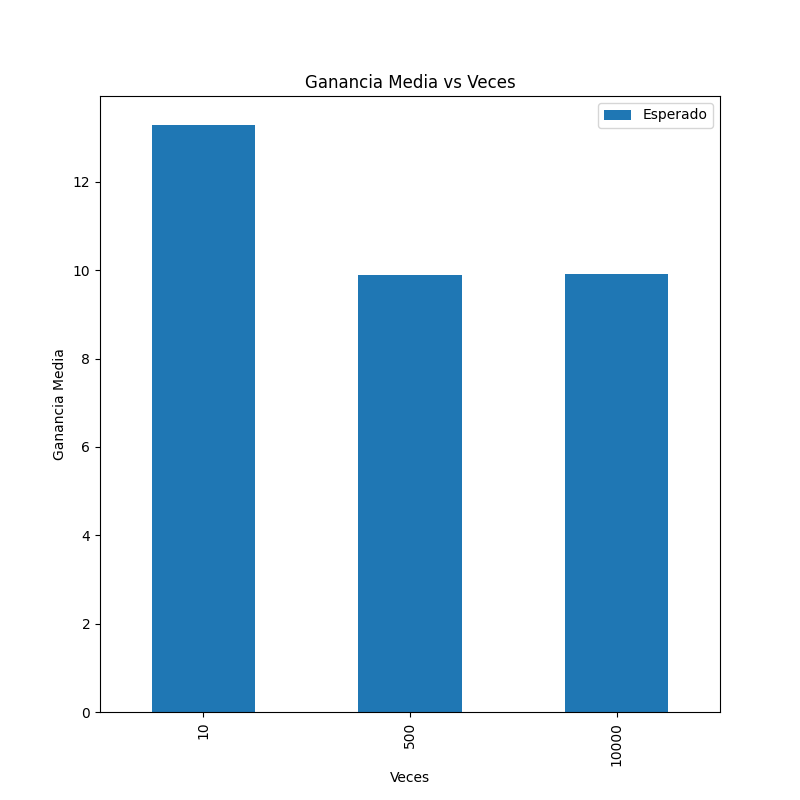
\includegraphics[width=0.5\textheight]{img/Cap-1/1-ganancia-media-vs-veces.png}
\end{center}

En ésta gráfica tenemos representada la media de ganancia esperada por cada vez que jugamos al juego un determinado número de veces. Podemos observar cómo el jugador se beneficia de jugar un número de veces reducido y se penaliza más al jugar un número de veces mayor que 10: mientras que jugando 10 veces seguidas consigue una media de más de 12, cuando jugamos 500 o 10000 veces seguidas ganamos menos de 10 euros de media. Ésto nos indica que si jugamos pagando 10 euros por tirada, y por cada partida completada nos dan 100 euros, debemos jugar un número de veces que ronde las 10 veces.

\section{Simulación alterando 'y' y 'z'}
Vamos a ver qué le ocurre al sistema si variamos los valores de pago por partida y de pago al finalizar cada partida para ver cuáles serán los beneficios o pérdidas del jugador.

\begin{center}
	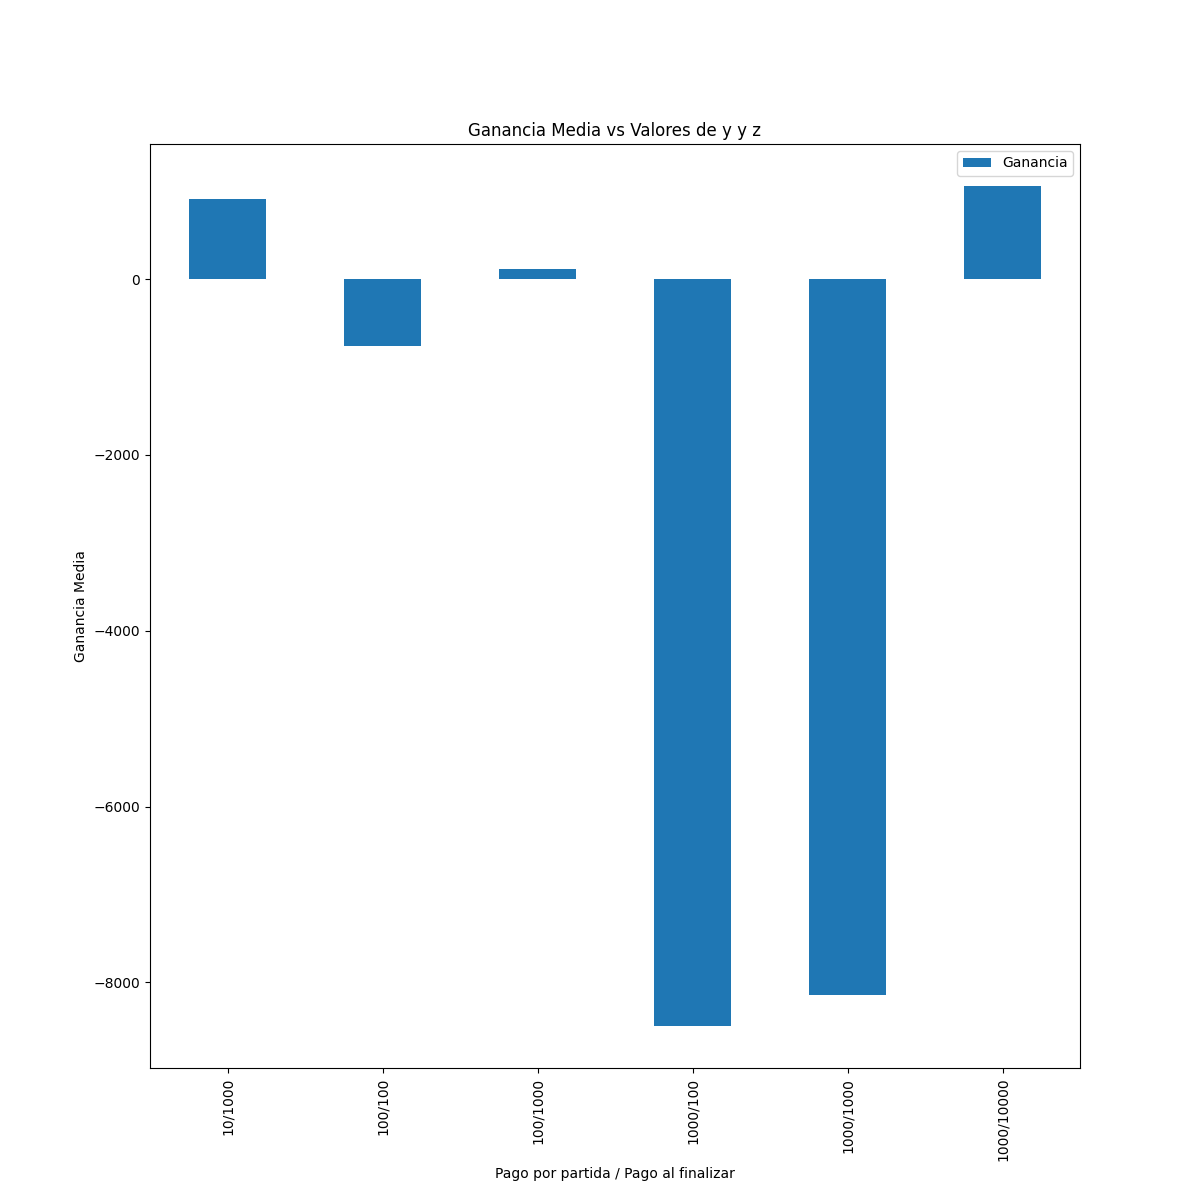
\includegraphics[width=0.6\textheight]{img/Cap-1/2-ganancia-media-vs-y-z.png}
\end{center}

Para llevar a cabo la simulación hemos usado los valores que aparecen en el eje x, que como se indica en dicho eje, el primero de ellos corresponde a la cantidad que hay que pagar para jugar y el segundo al pago que se recibe al finalizar el juego.

Al mantener la dinámica del juego de que termina cuando llegamos a obtener 3 veces seguidas o cara o cruz, es lógico que no merece la pena jugar cuando el pago por cada tirada es mucho mayor al pago que obtenemos al finalizar ya que en el caso más favorable (salgan 3 veces seguidas cara/cruz en las 3 primeras tiradas) ya perderíamos dinero.

Un caso más equilibrado es aquel en el que por cada tirada pagamos un 10\% de lo que ganaríamos, como es el caso del planteamiento del sistema o el del pago de 100 por tirada y pago al finalizar de 1000 como se ve en la gráfica.

Podemos observar también como en la primera y la última barra obtenemos mucho más que en el caso inicial, debido a que el pago por tirada es mucho menor que el pago al finalizar en ambos casos. Por lo tanto si nos ofreciesen jugar con dichas condiciones es muy probable que consigamos beneficio.
\newpage
\section{Cambios en los parámetros de probabilidad y diferencia}
\subsection{Pruebas con la probabilidad}
En este caso, vamos a ver cómo afecta al sistema que truquemos de la moneda, consiguiendo muchas más cruces que caras o más caras que cruces. En el siguiente gráfico se encuentra representada la gráfica relativa a la ganancia media en función de la probabilidad relativa a la moneda:

\begin{center}
	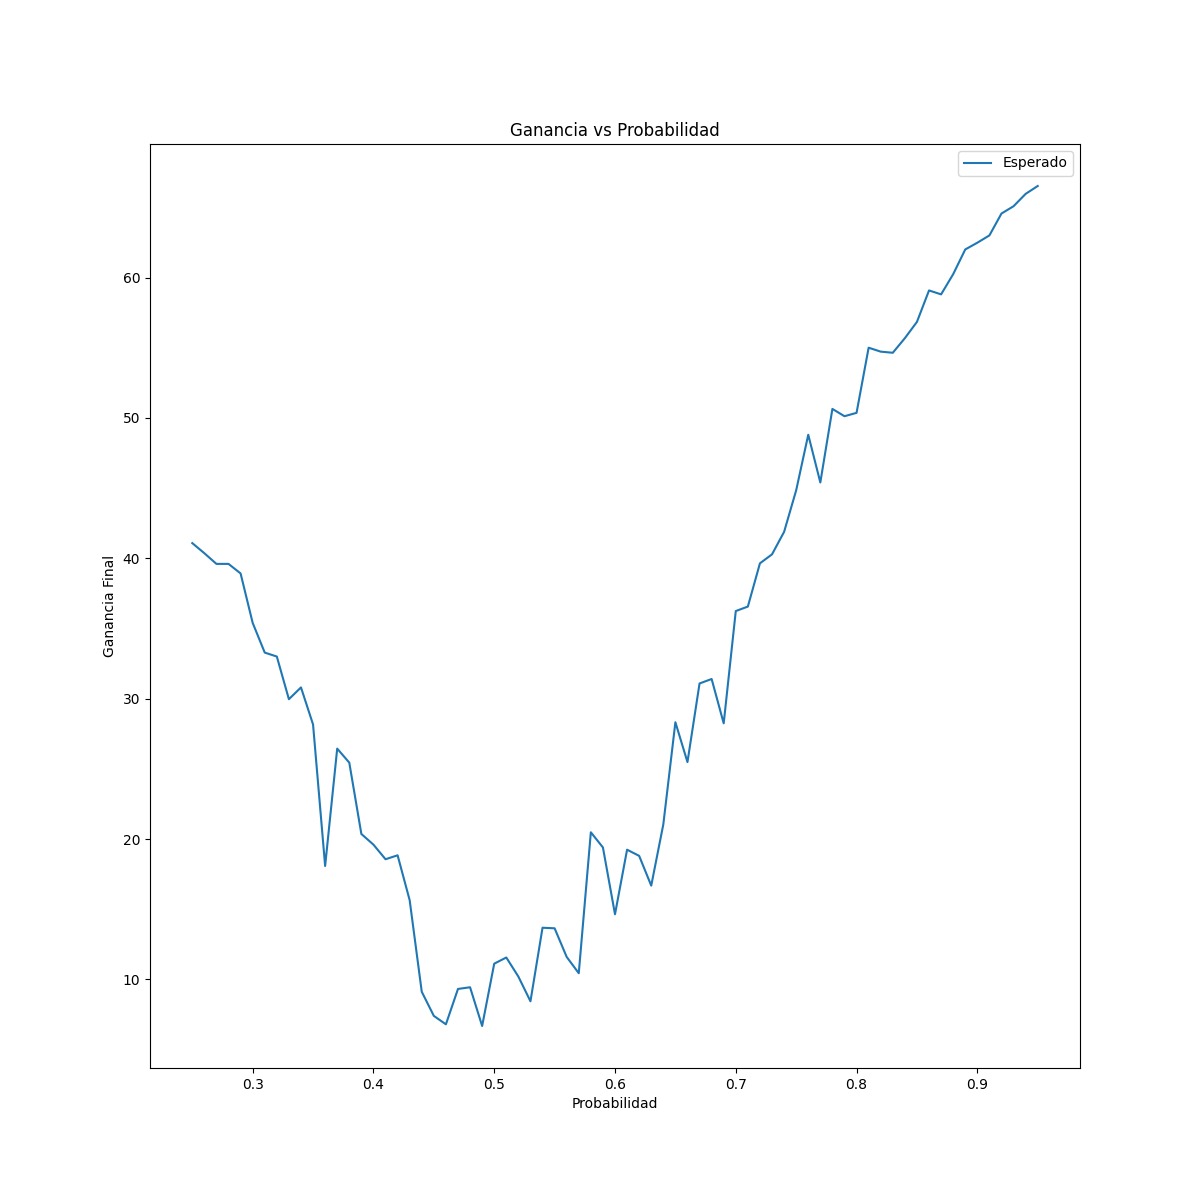
\includegraphics[width=0.6\textheight]{img/Cap-1/3-ganancia-vs-probabilidad.png}
\end{center}

En ésta gráfica se puede ver cómo hay un valle en la ganancia media cuando probabilidad se acerca al valor de 0.5, debido a que si tenemos una probabilidad cercana a 1 o a 0.3 van a salir más cara o cruz (en función de a la probabilidad de la que nos estemos refiriendo). Éste gráfico es bastante obvio ya que cuanta más probabilidad tengamos de que salga una u otra, más ganancia media obtendremos, mientras que cuando haya la misma probabilidad de que obtengamos cara o cruz, la ganancia es menor.
\newpage
\subsection{Pruebas con la diferencia}

Lo siguiente que probaremos va a ser variar el número de veces que tienen que salir repetidas una de las caras de la moneda para finalizar el juego. Simulando el sistema para distintos valores de la diferencia obtenemos el siguiente gráfico:

\begin{center}
	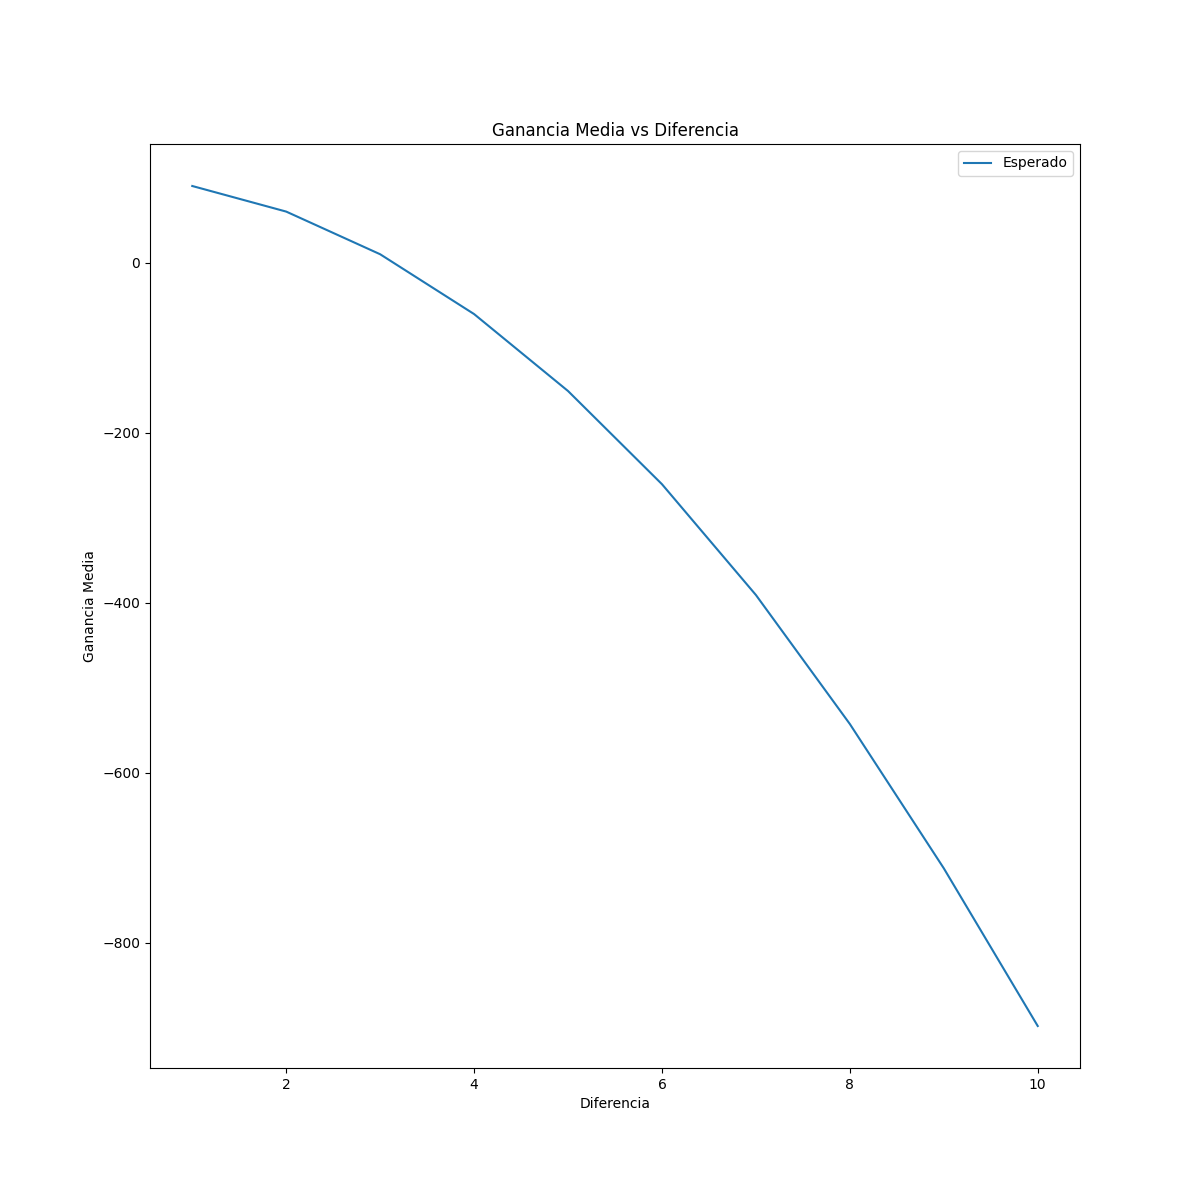
\includegraphics[width=0.6\textheight]{img/Cap-1/3-ganancia-media-vs-diferencia.png}
\end{center}

Podemos observar que la ganancia media pasa a ser negativa en el momento que nos pasamos de 3. La conclusión que podemos obtener con respecto a la diferencia del número de caras y cruces es que empieza a no ser rentable a partir de 3 de diferencia ya que como se puede ver en la gráfica, los valores pasan a ser muy negativos desde el momento que bajamos de dicho valor.

\subsection{Pruebas variando dos parámetros a la vez}

La última simulación que he realizado con el sistema propuesto es qué conclusiones podemos obtener si variamos tres parámetros a la vez a la hora de ejecutar. Para ello lo que he hecho ha sido variar tanto la probabilidad como la diferencia de caras y cruces a la vez para ver qué situación puede beneficiarnos más. La siguiente gráfica muestra los datos obtenidos en la prueba comentada:

\begin{center}
	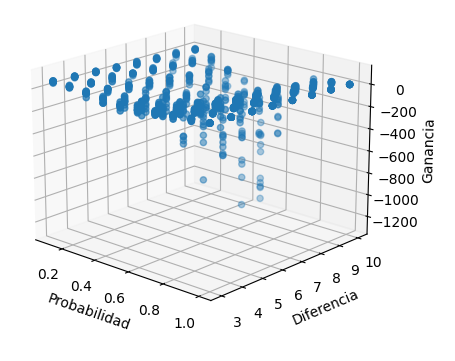
\includegraphics[width=0.6\textheight]{img/Cap-1/3-ganancia-vs-prob-vs-diff.png}
\end{center}

En ésta podemos ver que la situación más favorable (en la que obtenemos mayor ganancia) es cuando nos acercamos a la punta más cercana a nosotros. Es decir, los valores donde la diferencia de caras y de cruces es más cercana a 3, y en los extremos de la probabilidad como hemos comentado en el apartado anterior.

\chapter{Mi primer Modelo de Simulación Discreto}
\newpage
\section{Inventario 1}
En ésta simulación tenemos que comprobar cuál es la mejor política estacionaria de las que se proponen en el guión. He realizado la simulación con los valores que se proponen probando diferentes número de veces y he obtenido varias gráficas al respecto las cuales se muestran a continuación:

\begin{center}
	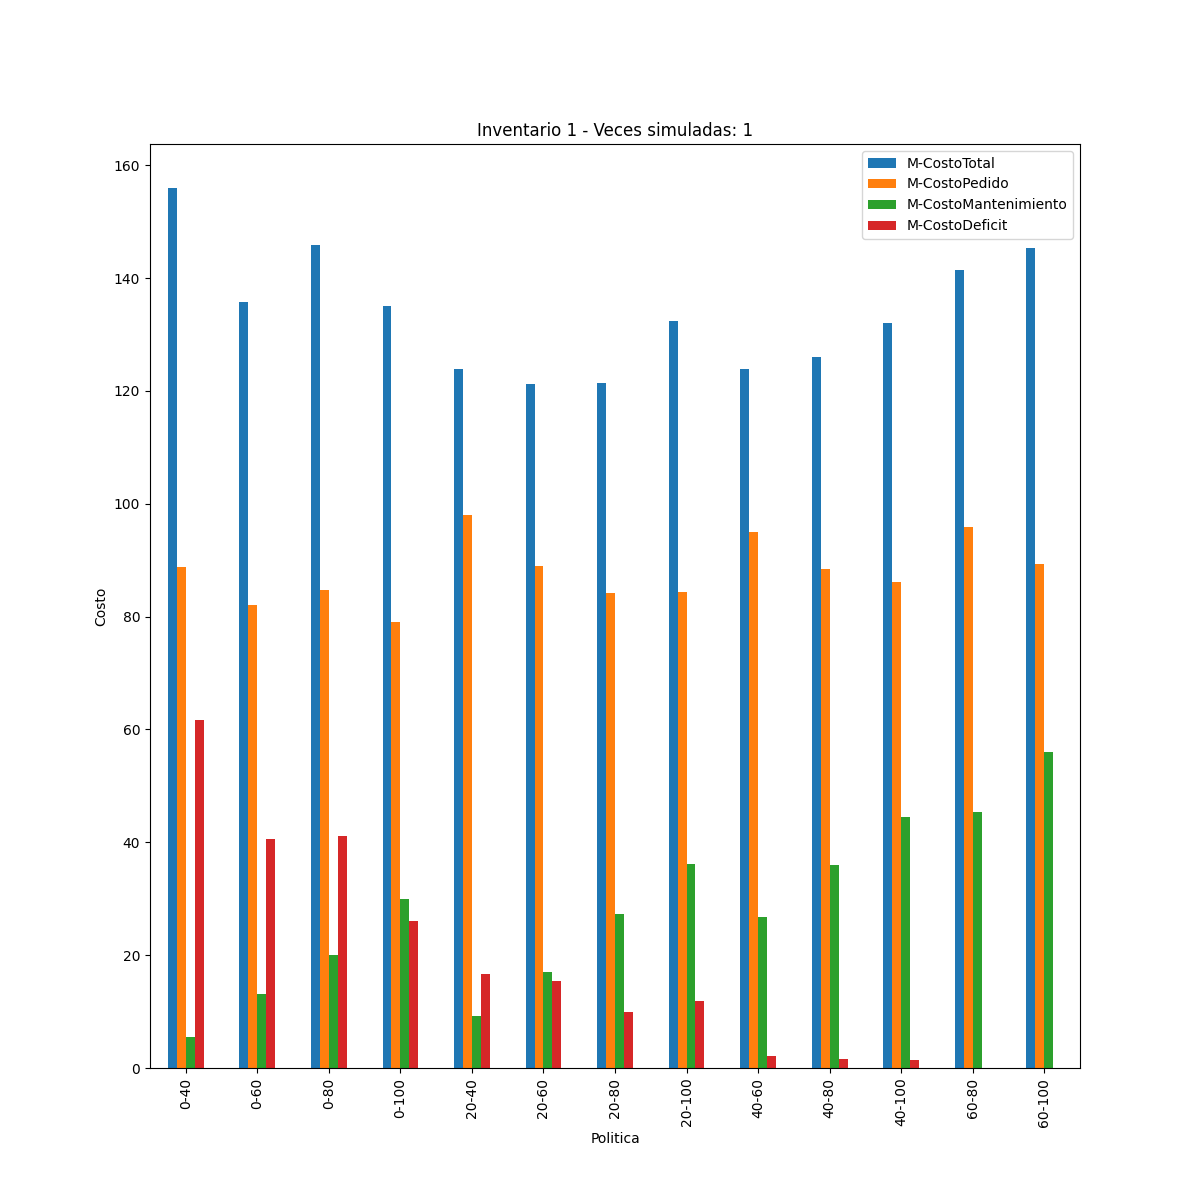
\includegraphics[width=0.4\textheight]{img/Cap-2/inventario-1/inventario1-1veces.png}
	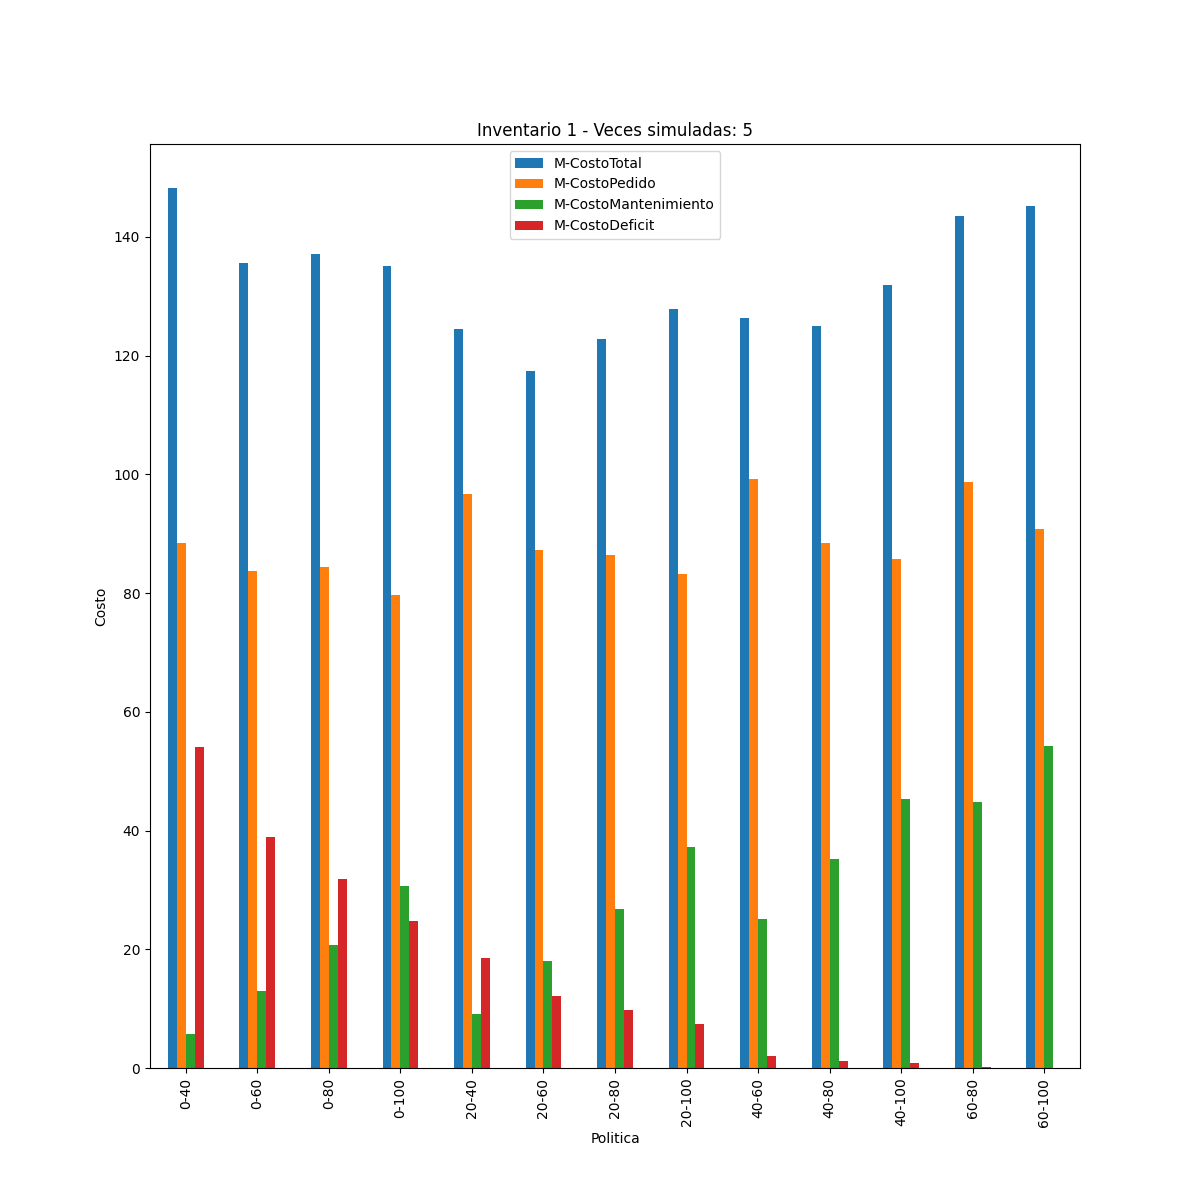
\includegraphics[width=0.4\textheight]{img/Cap-2/inventario-1/inventario1-5veces.png}
	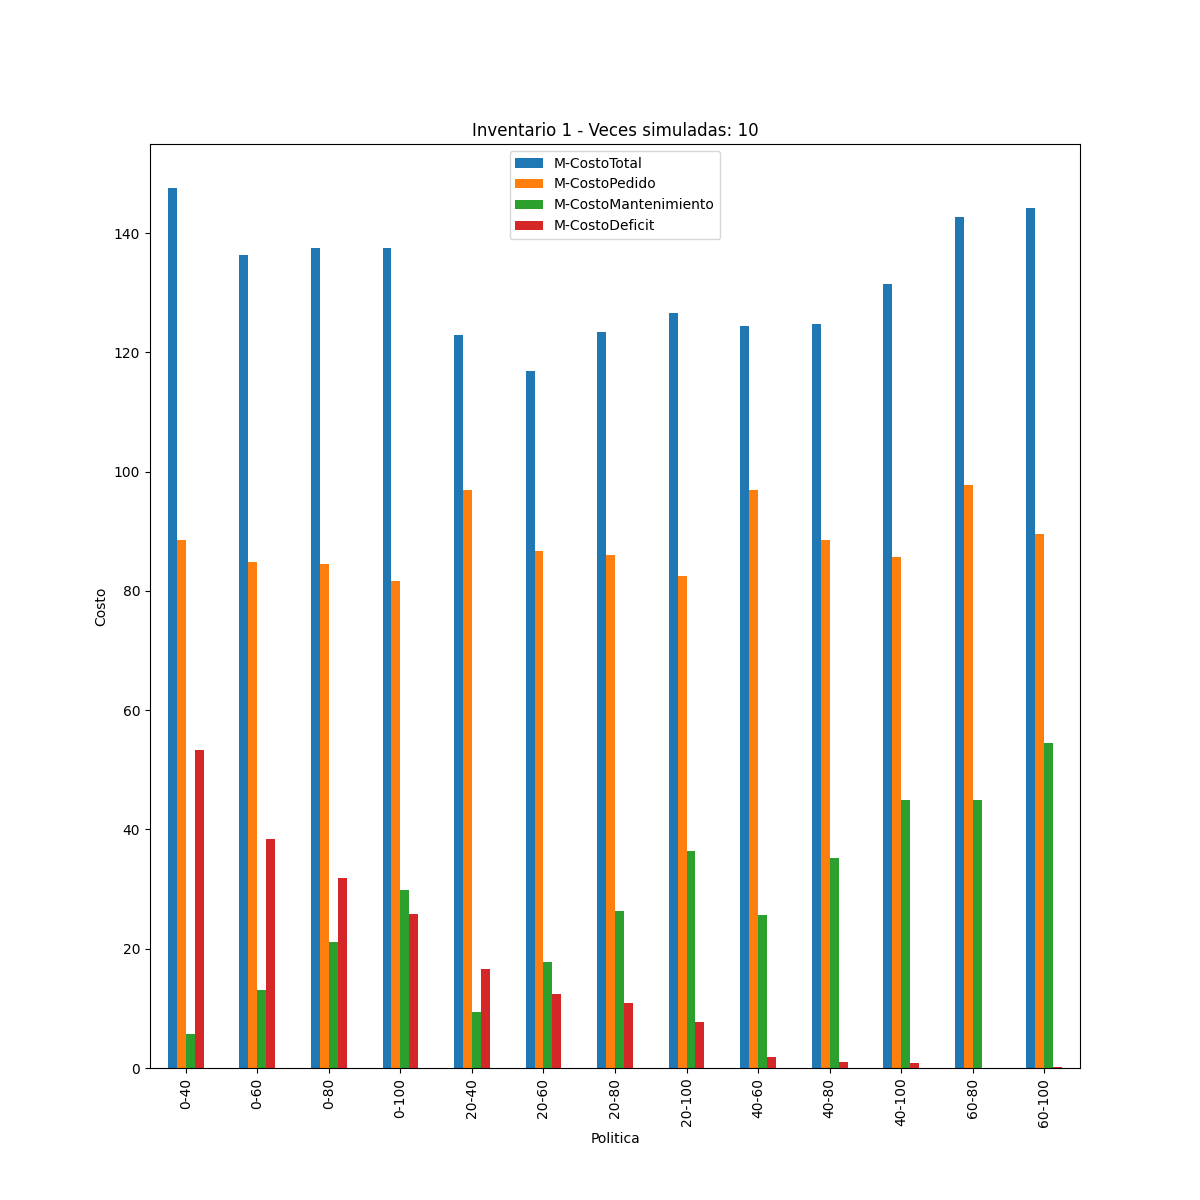
\includegraphics[width=0.45\textheight]{img/Cap-2/inventario-1/inventario1-10veces.png}
	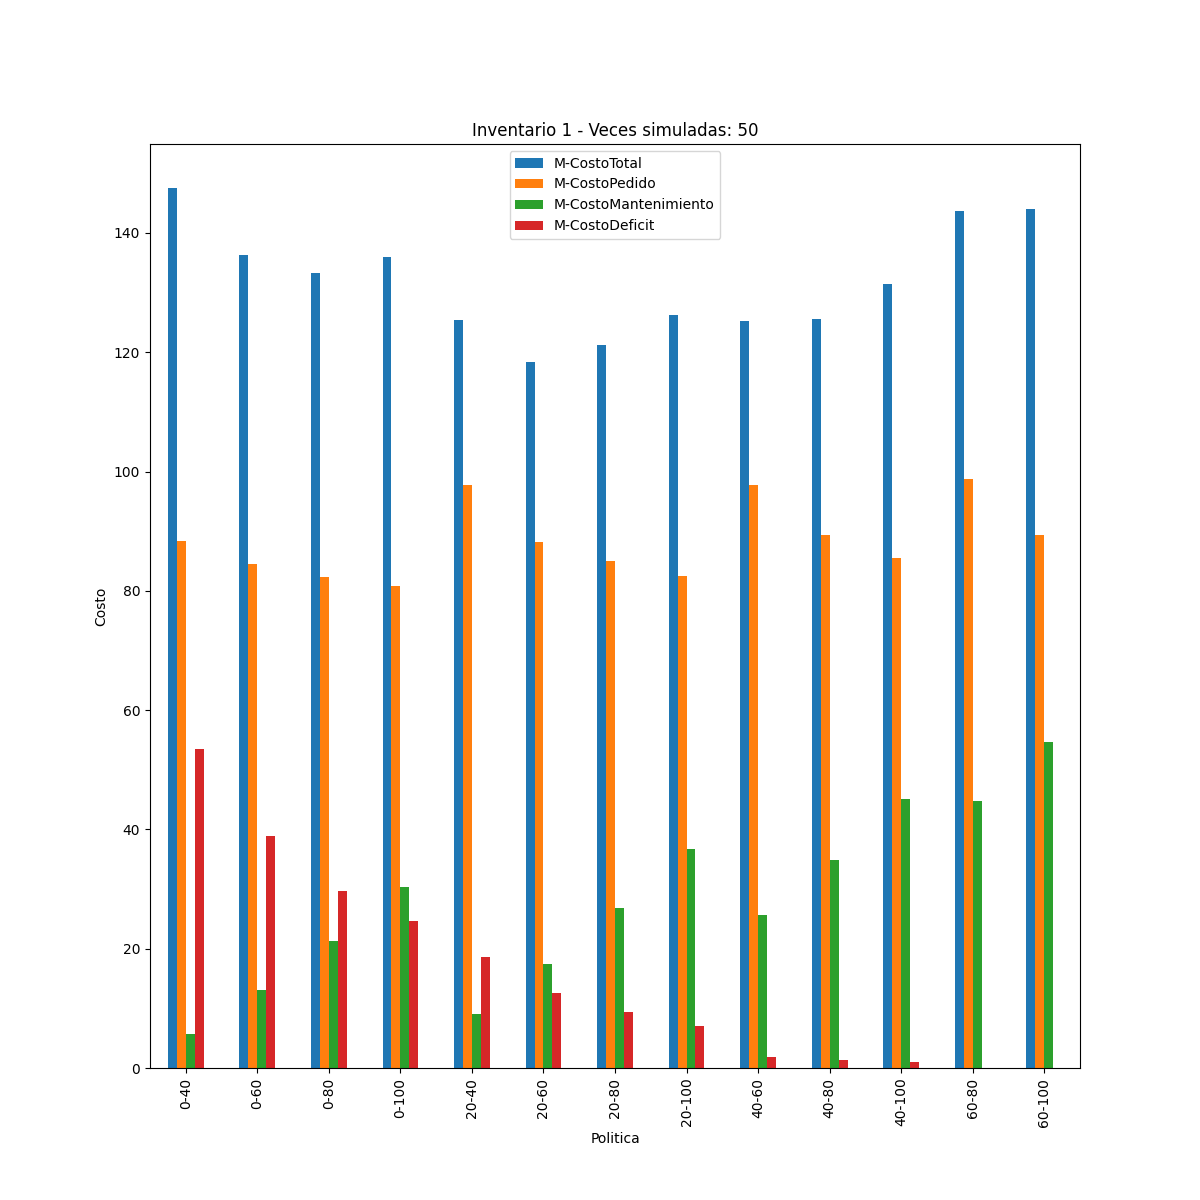
\includegraphics[width=0.45\textheight]{img/Cap-2/inventario-1/inventario1-50veces.png}
	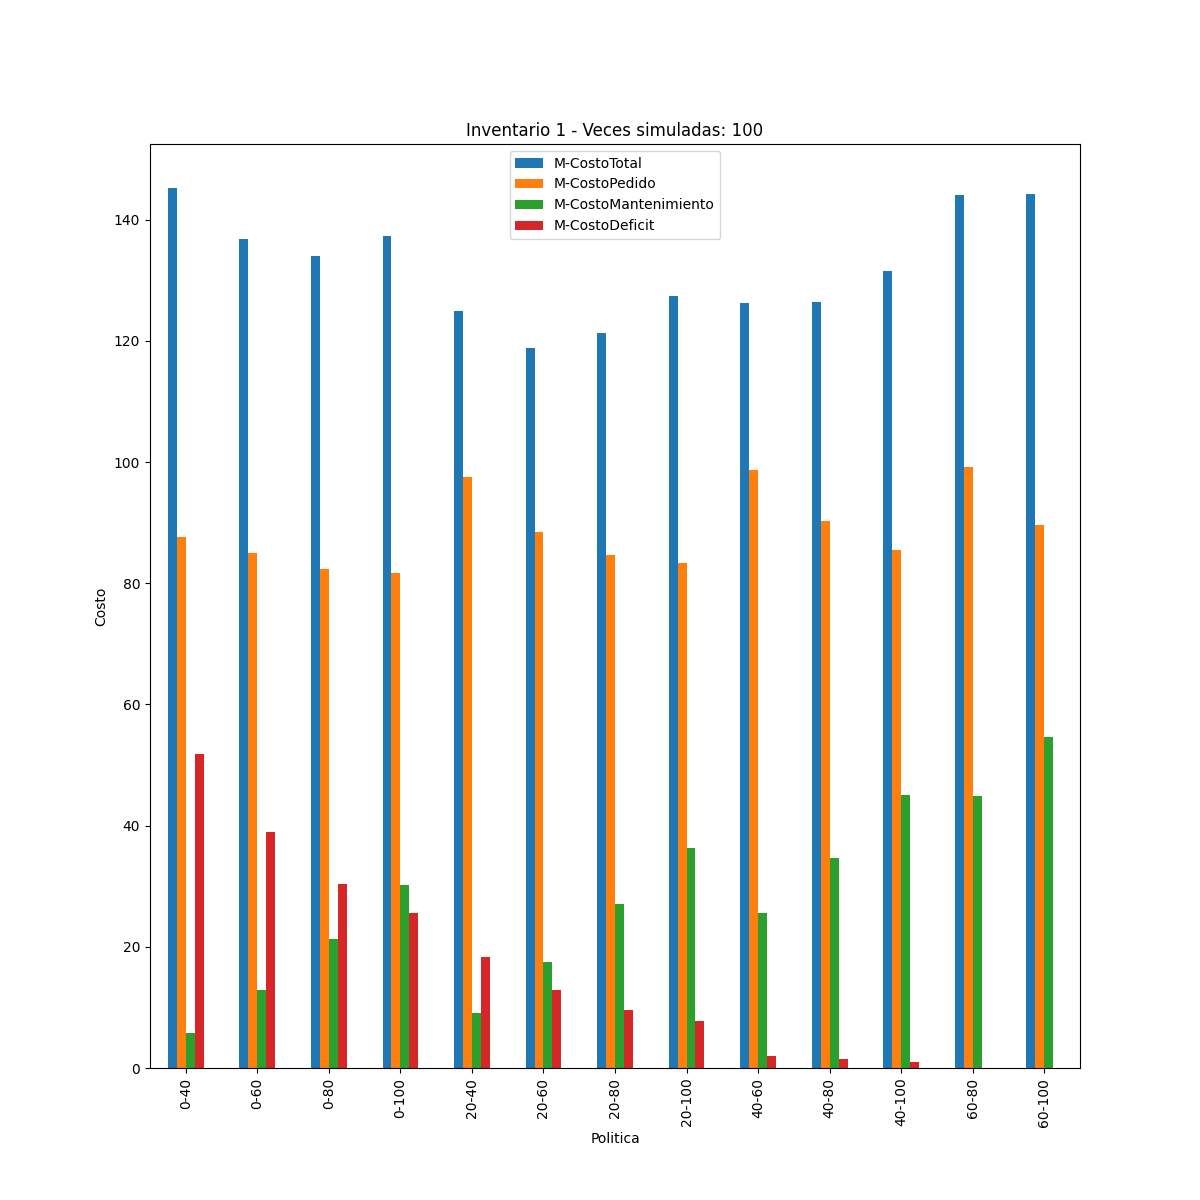
\includegraphics[width=0.45\textheight]{img/Cap-2/inventario-1/inventario1-100veces.png}
	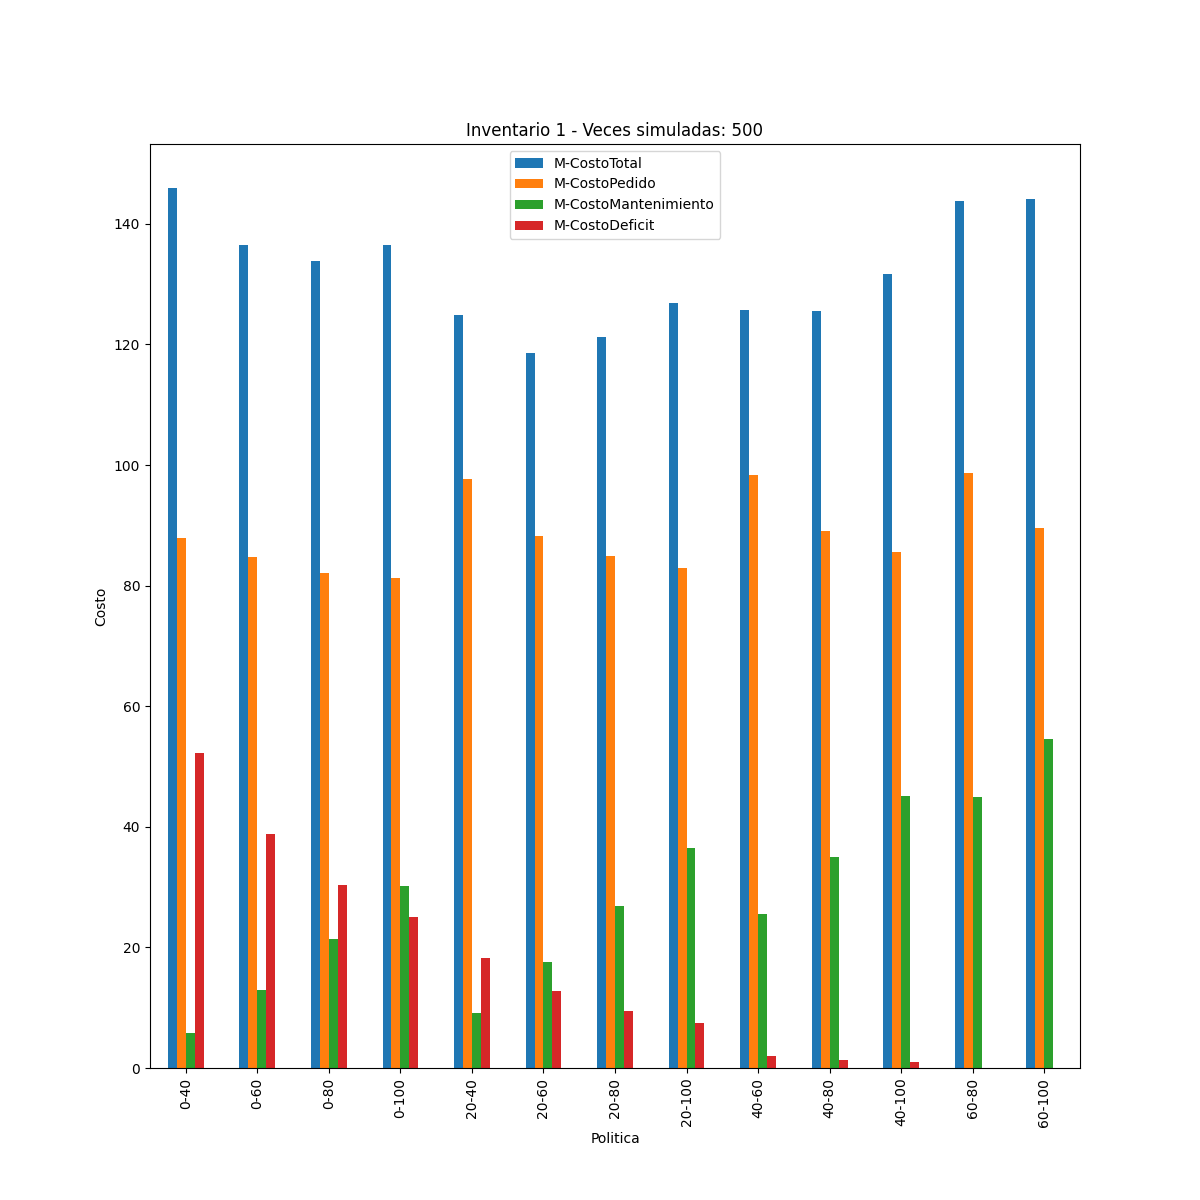
\includegraphics[width=0.45\textheight]{img/Cap-2/inventario-1/inventario1-500veces.png}
\end{center}

Se puede apreciar muy levemente cómo a medida que aumentamos el número de simulaciones, los valores obtenidos empiezan a ser más precisos y obtenemos una media más concreta. 
La conclusión que podemos sacar a partir de la ejecución del inventario 1 500 veces es que la política con s=20 y S=60 es la mejor política debido a que es la política en la que tenemos un costo total menor que el resto.

\section{Inventario 2}

\begin{center}
	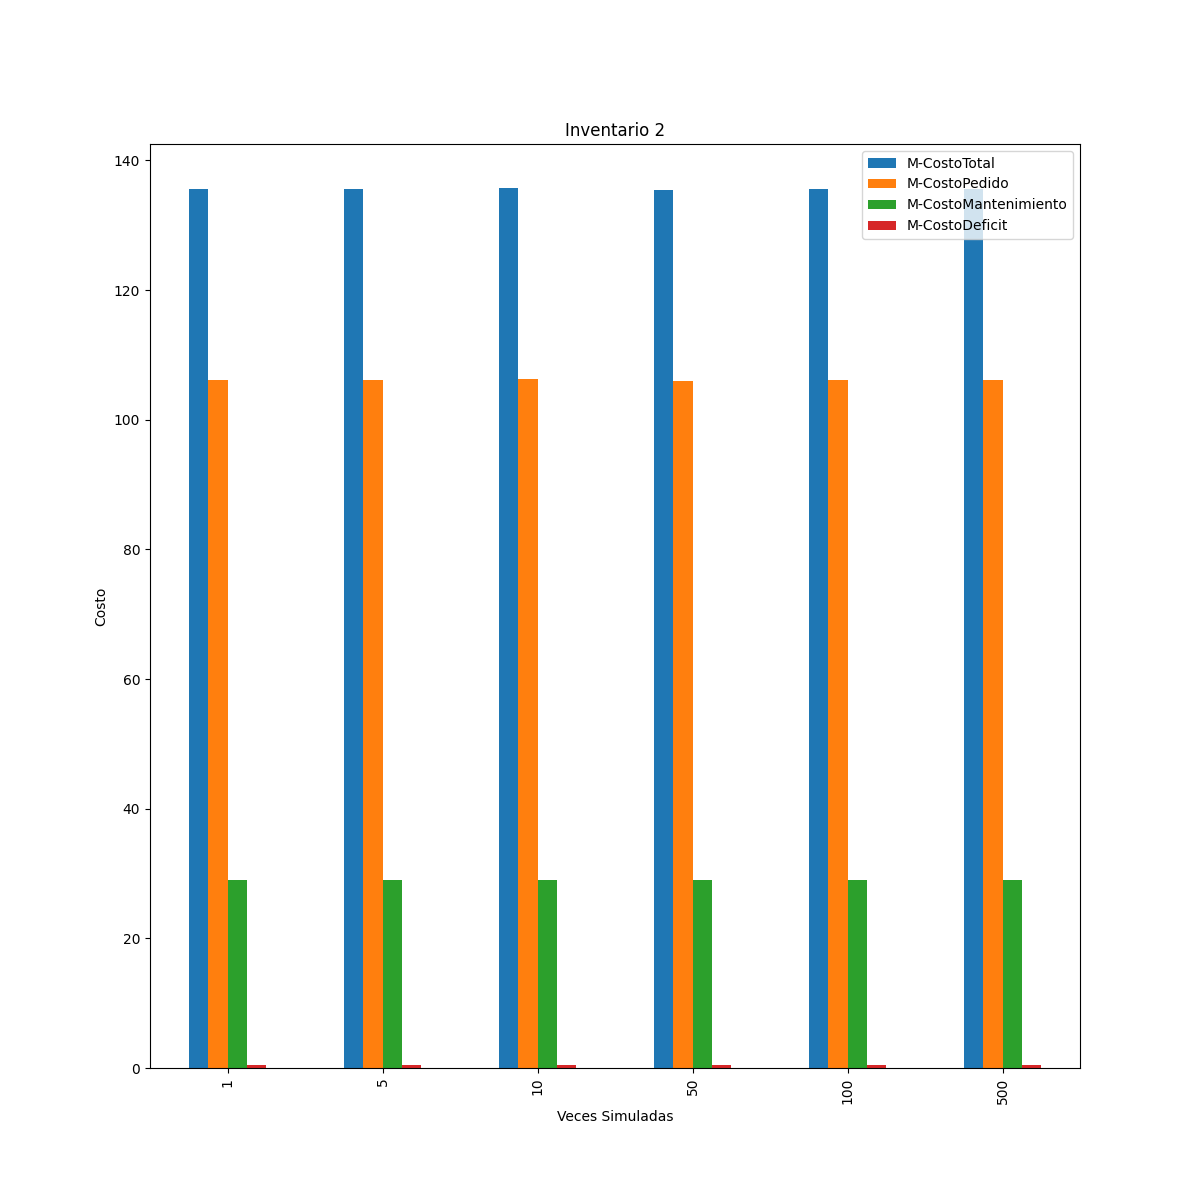
\includegraphics[width=0.45\textheight]{img/Cap-2/inventario-2/inventario2.png}
\end{center}

De la simulación del inventario 2 hemos obtenido que 

\section{Inventario 3}
\begin{center}
	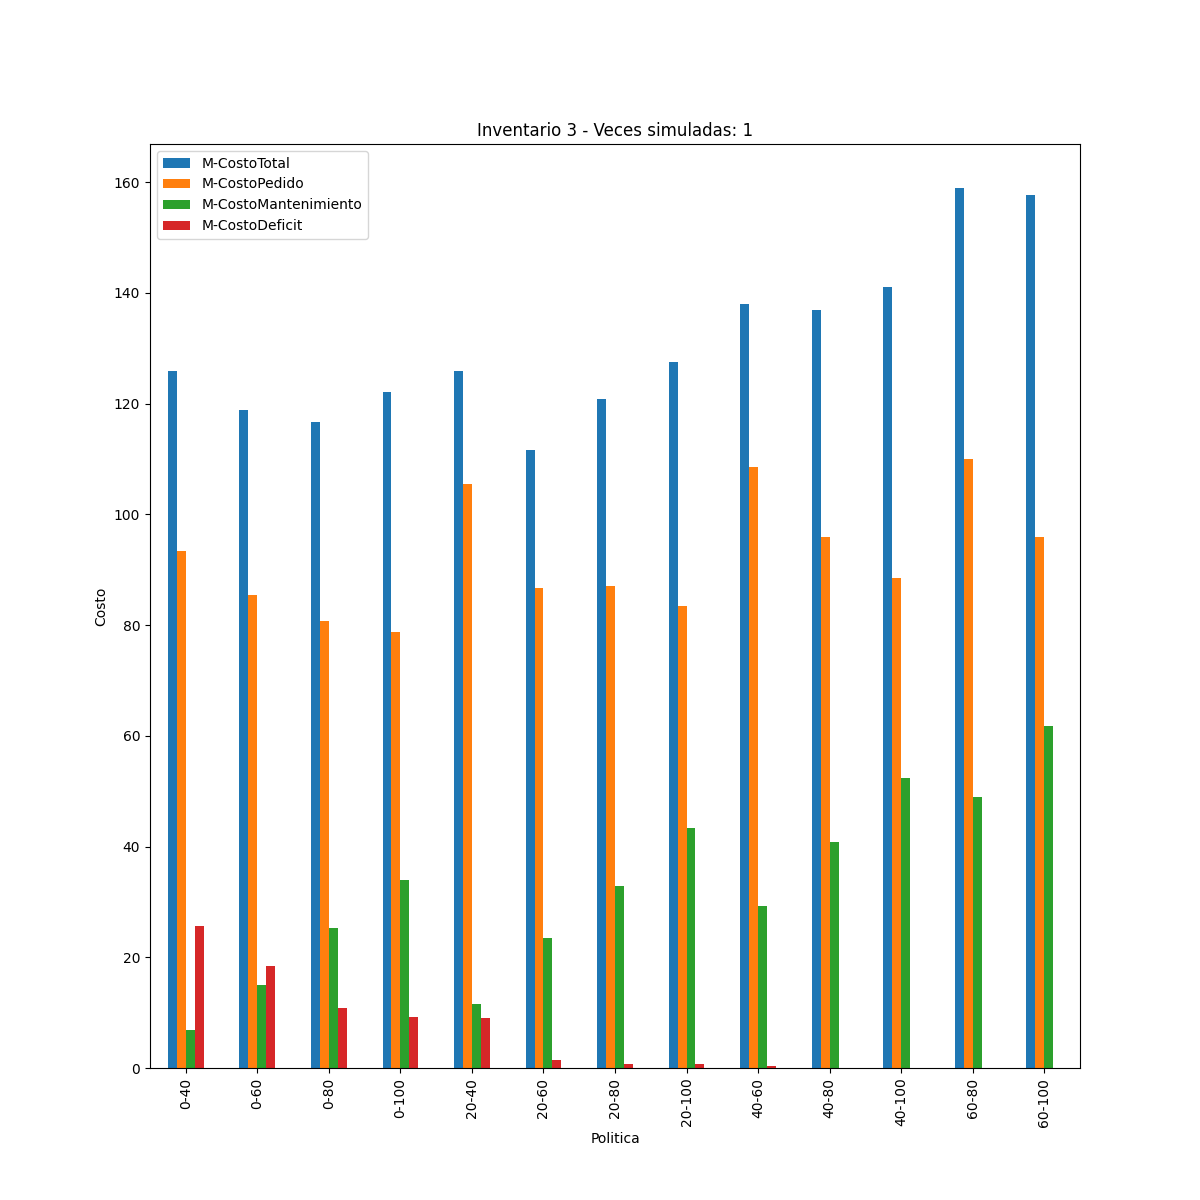
\includegraphics[width=0.4\textheight]{img/Cap-2/inventario-3/inventario3-1veces.png}
	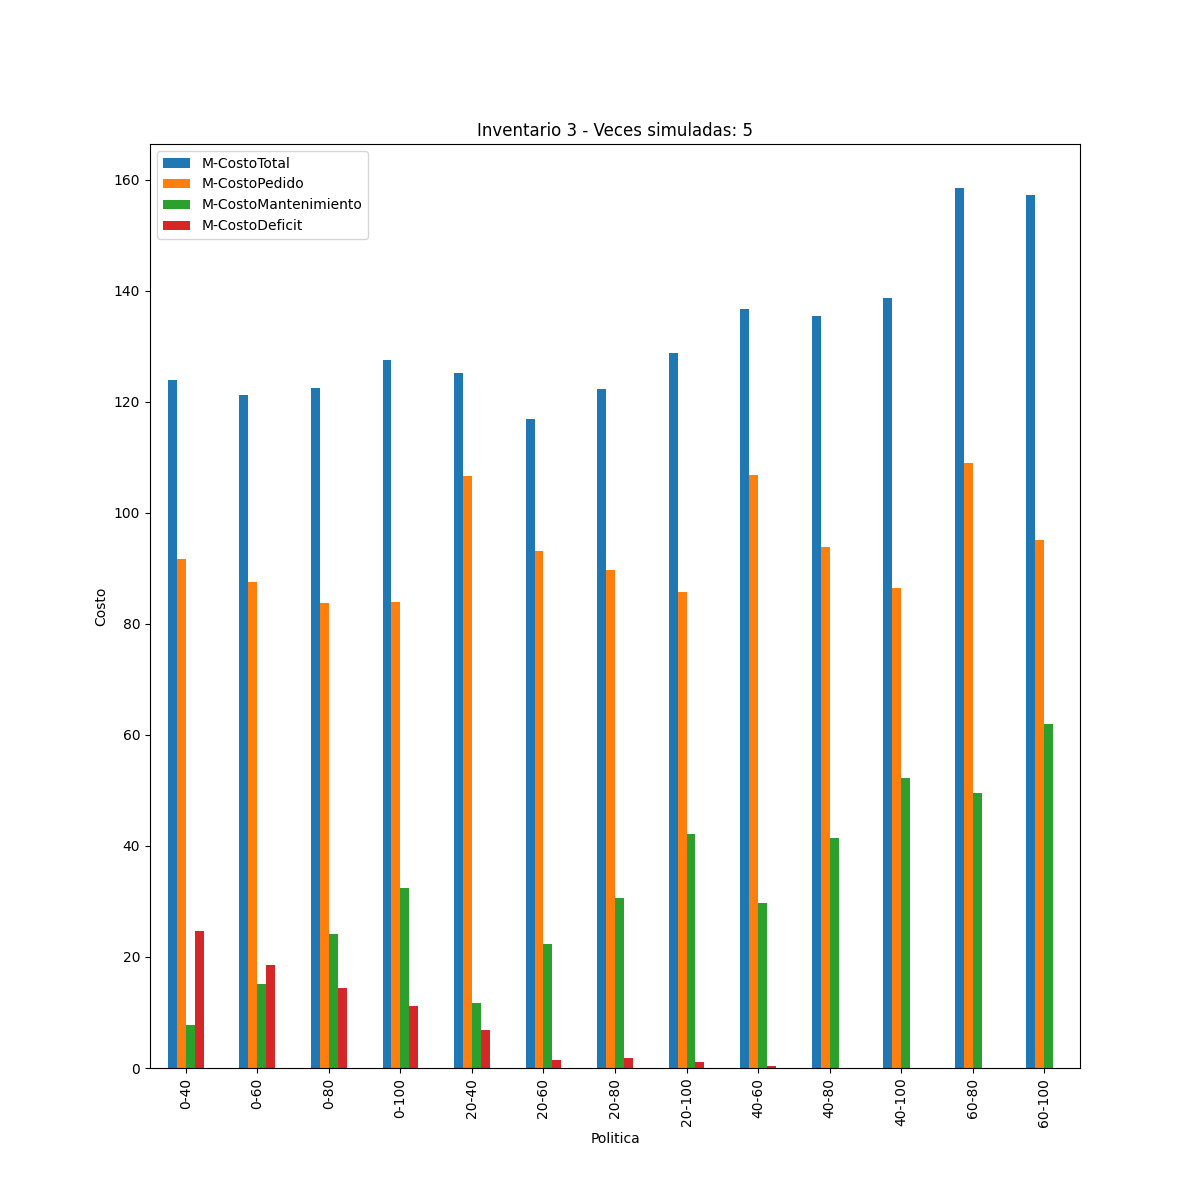
\includegraphics[width=0.4\textheight]{img/Cap-2/inventario-3/inventario3-5veces.png}
	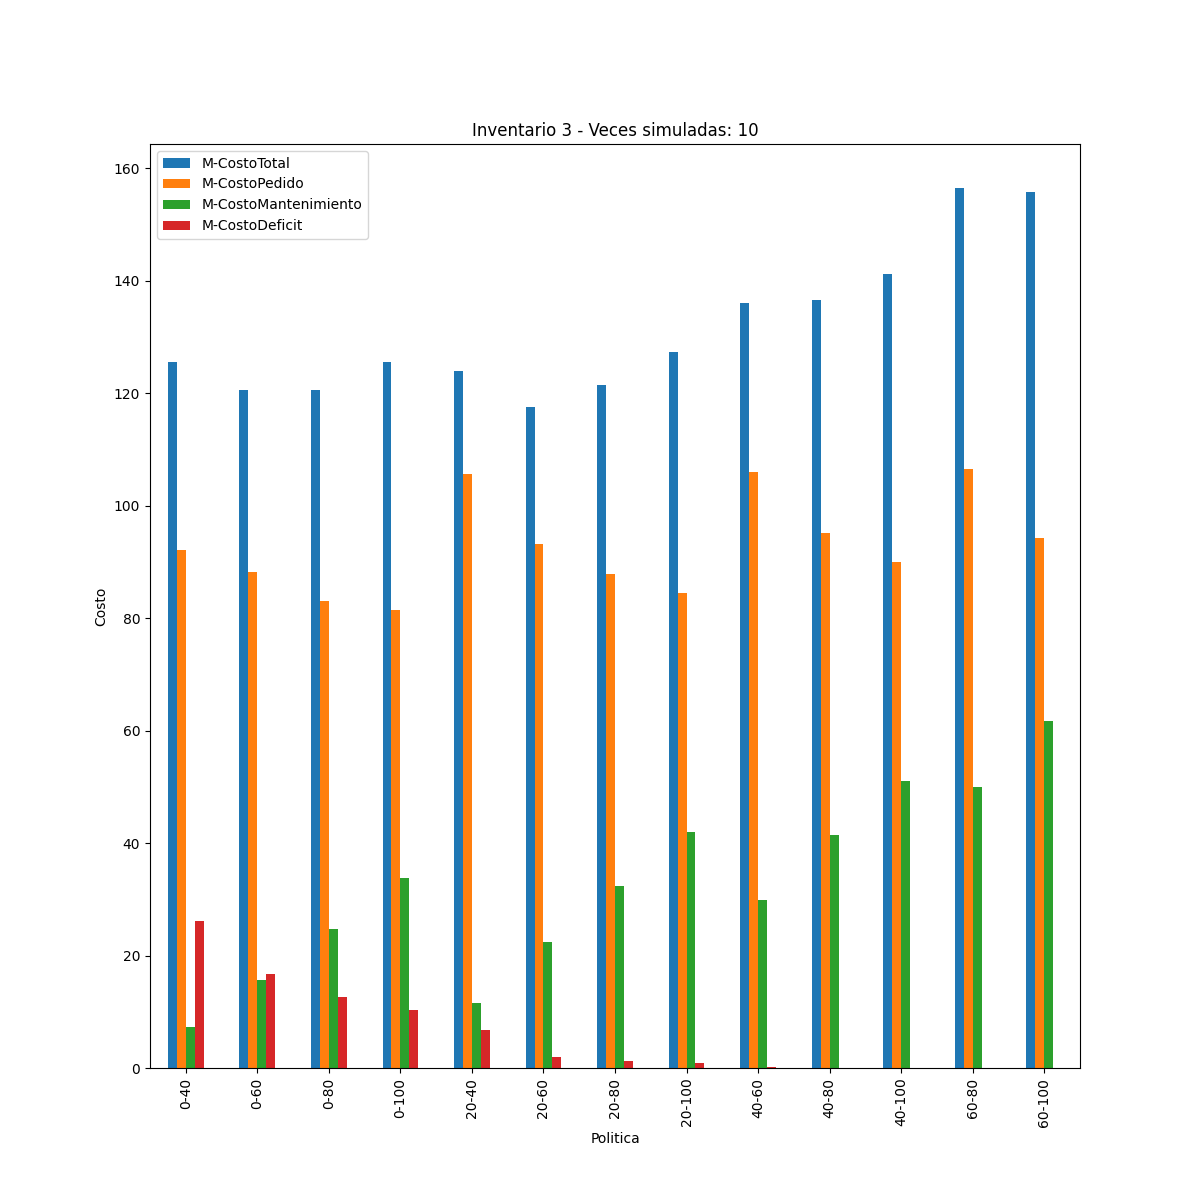
\includegraphics[width=0.45\textheight]{img/Cap-2/inventario-3/inventario3-10veces.png}
	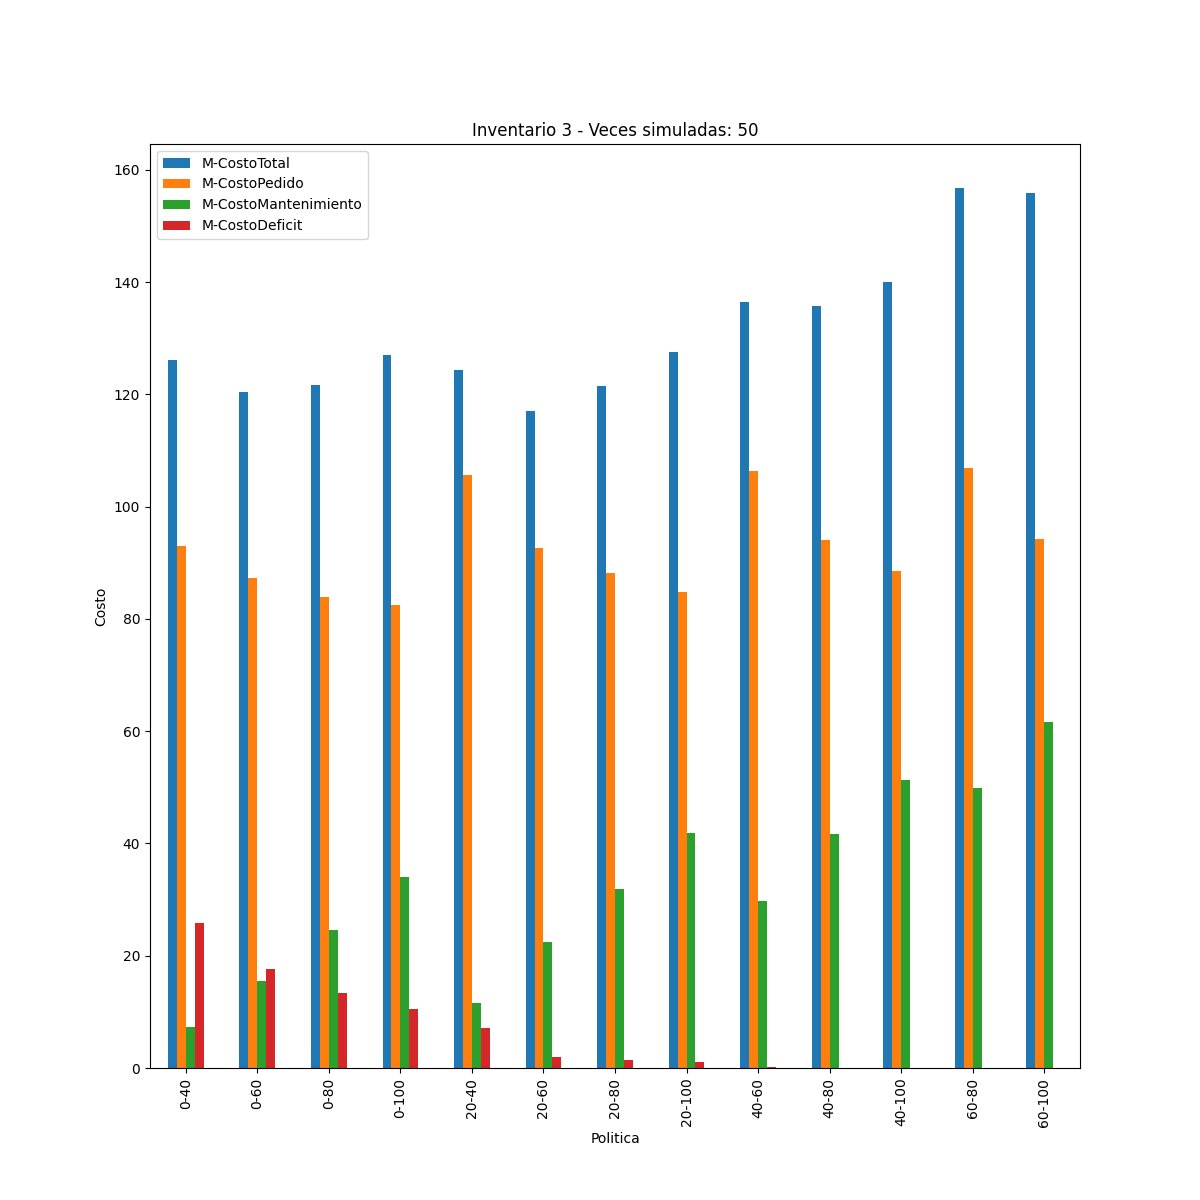
\includegraphics[width=0.45\textheight]{img/Cap-2/inventario-3/inventario3-50veces.png}
	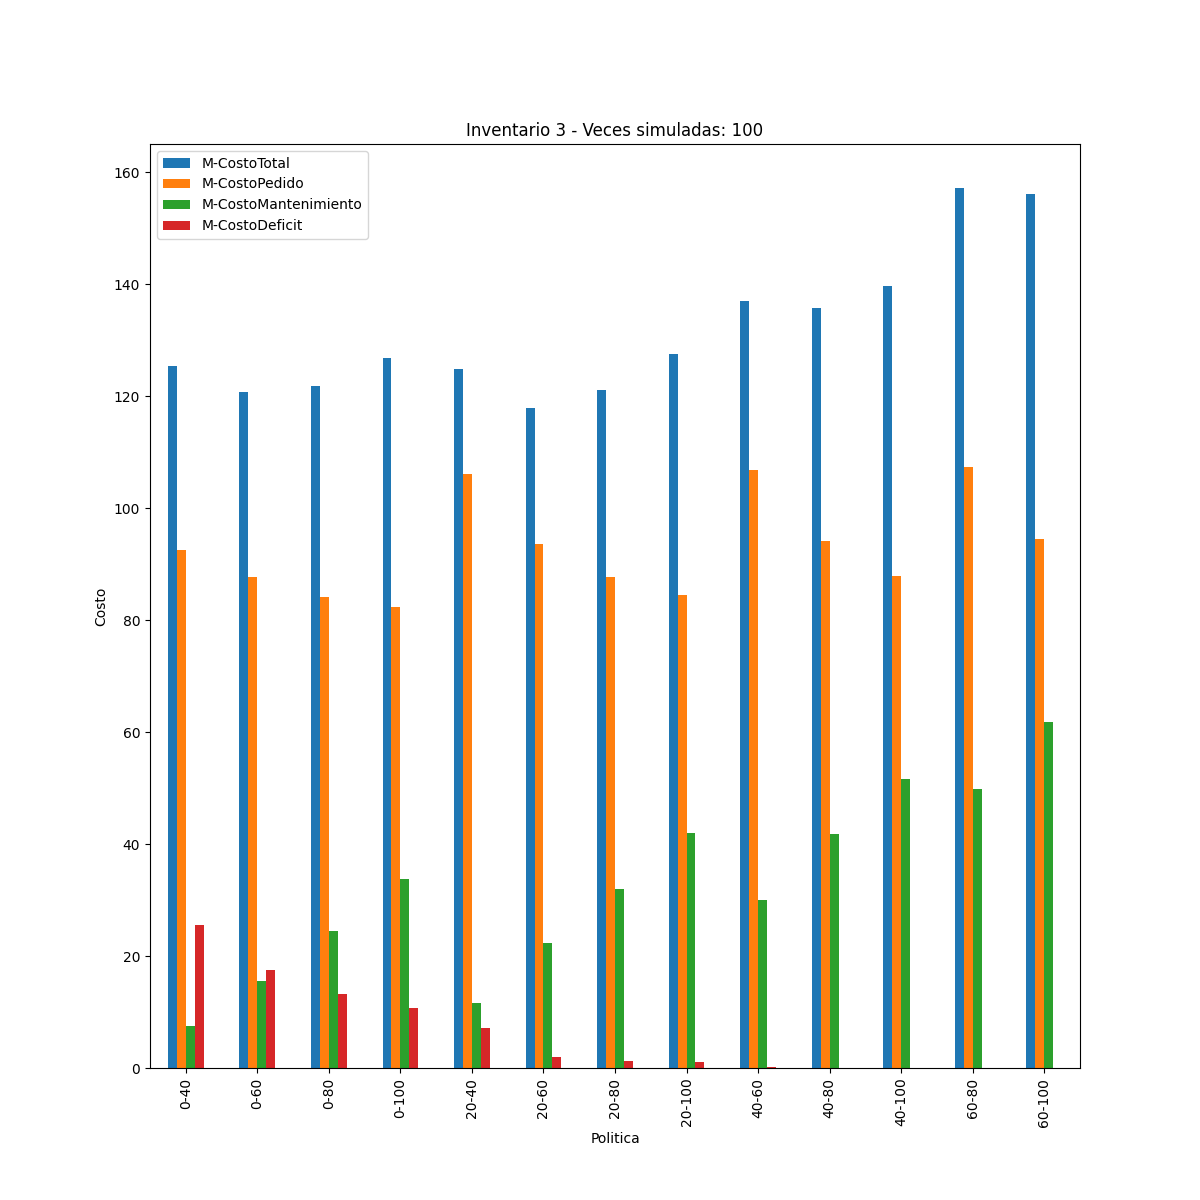
\includegraphics[width=0.45\textheight]{img/Cap-2/inventario-3/inventario3-100veces.png}
	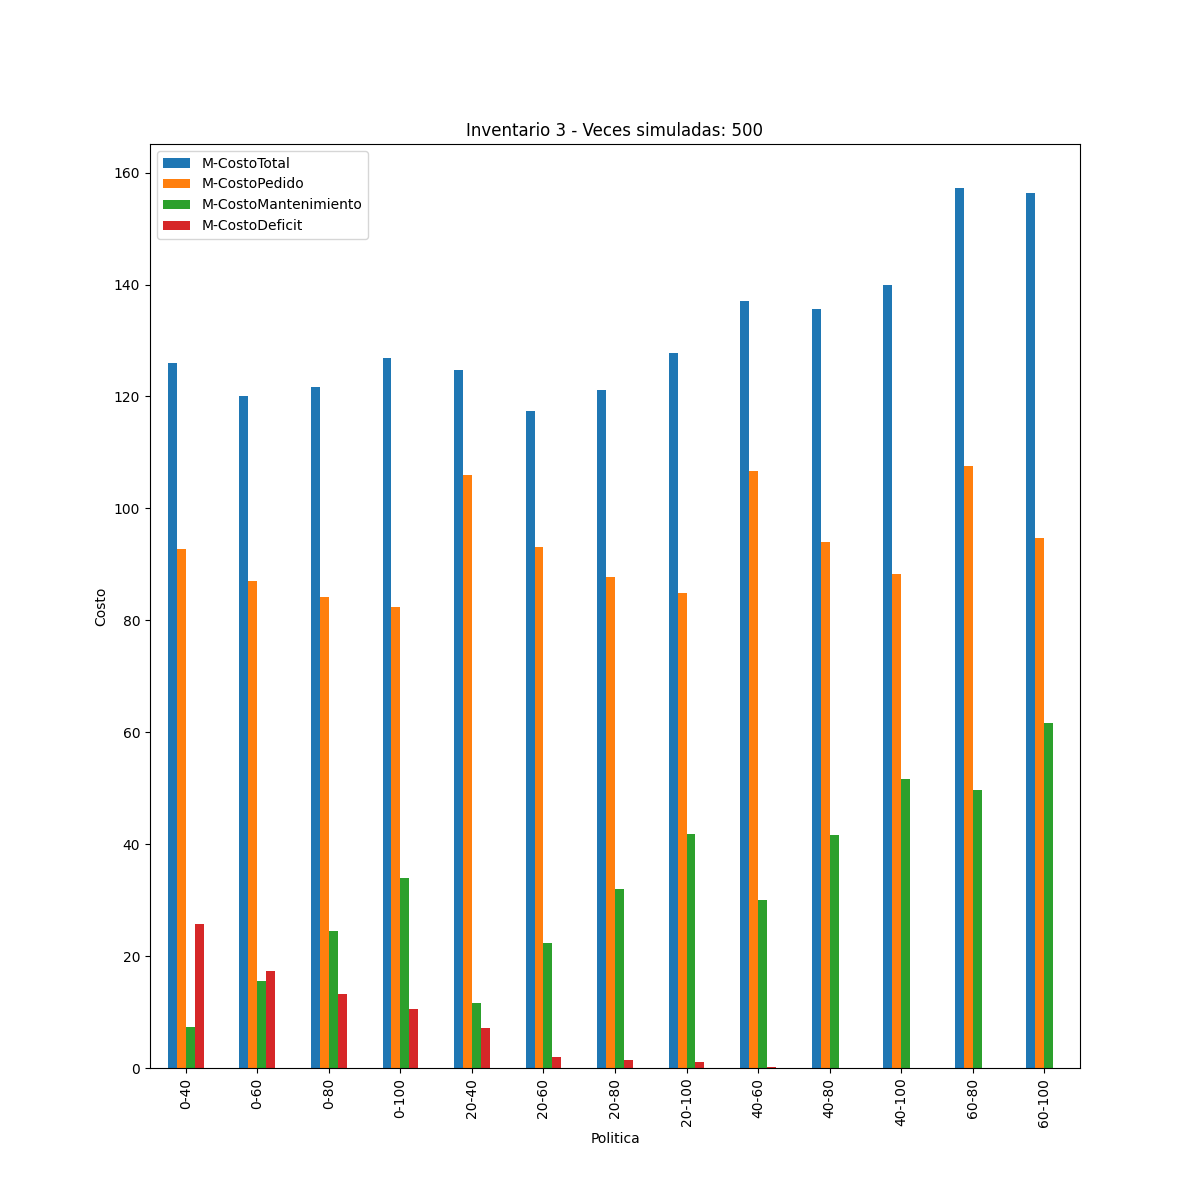
\includegraphics[width=0.45\textheight]{img/Cap-2/inventario-3/inventario3-500veces.png}
\end{center}

\newpage
\chapter{Mi primer Modelo de Simulación Continuo}
\newpage
\section{Punto de estabilidad del lago}
Para comprobar si es posible llegar a un punto de estabilidad en cuanto al número de especies que hay de peces grandes y peces pequeños, he probado con distintos valores y el resultado ha sido que he encontrado un caso en el que sí y otro en el que no. 

En el primer caso he simulado en 3000 días si 10000 peces pequeños y 200 peces grandes eran capaces de equilibrarse obteniendo los datos reflejados en la siguiente gráfica:

\begin{figure}[H]
  \begin{subfigure}[b]{0.49\textwidth}
    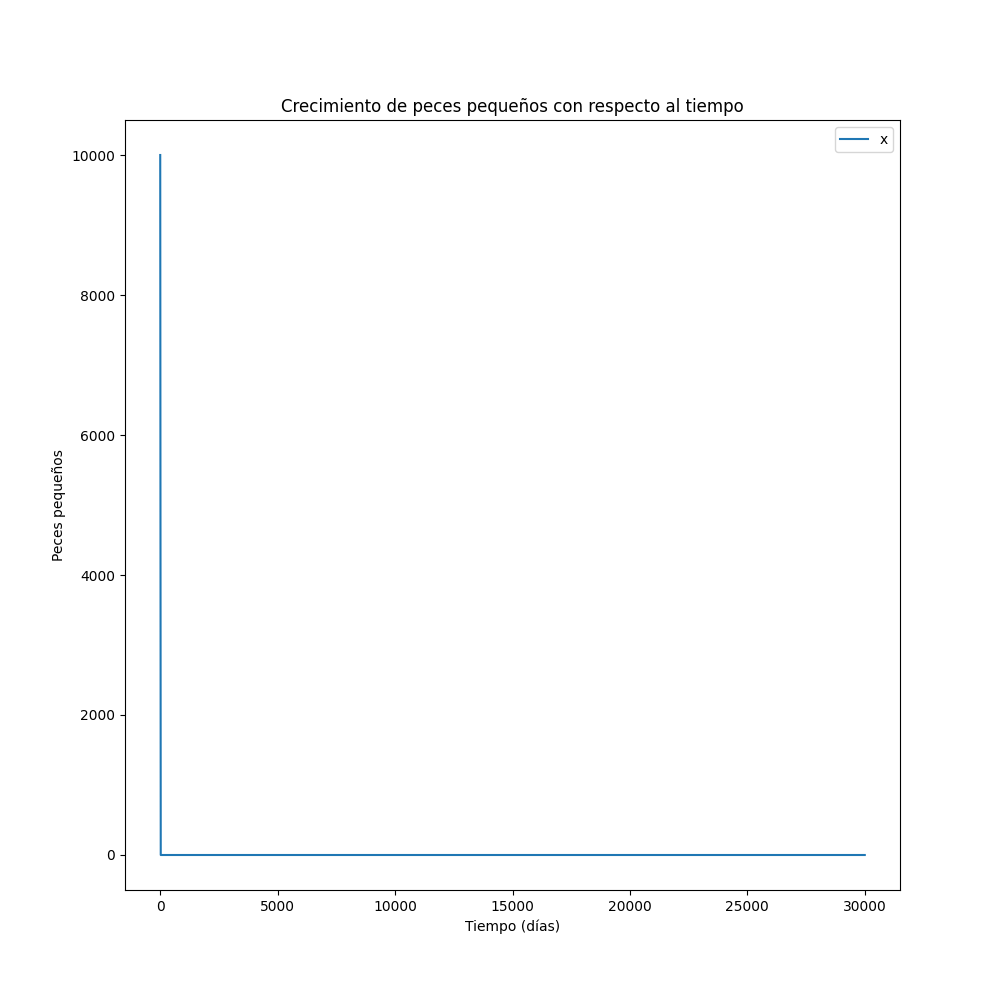
\includegraphics[width=\textwidth, height=\textwidth]{img/Cap-3/apartado-1/peces_pequenos_200.png}
    \caption{Crecimiento de peces pequeños.}
    \label{fig:f1}
  \end{subfigure}
  \hfill
  \begin{subfigure}[b]{0.49\textwidth}
    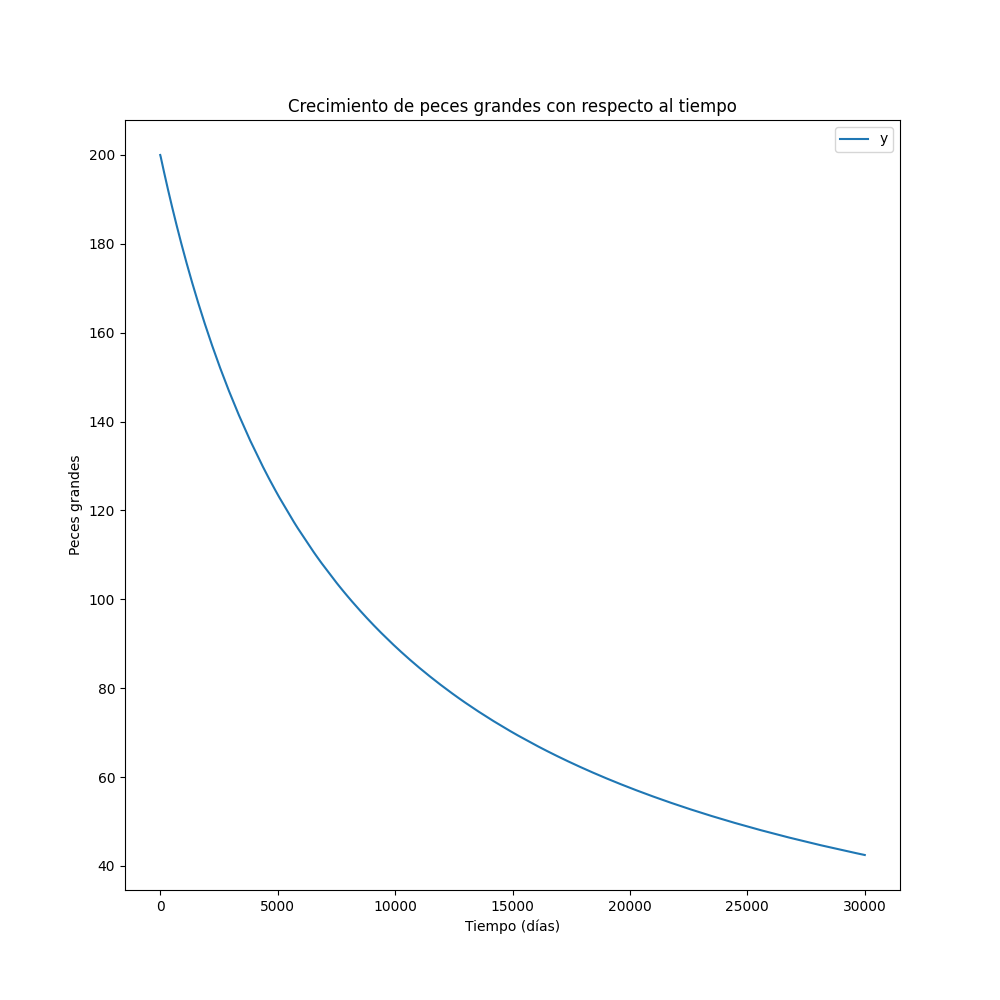
\includegraphics[width=\textwidth, height=\textwidth]{img/Cap-3/apartado-1/peces_grandes_200.png}
    \caption{Crecimiento de peces grandes.}
    \label{fig:f2}
  \end{subfigure}
  \caption{Crecimiento de especies del lago con 10000 peces pequeños y 200 peces grandes}
\end{figure}

Como podemos ver, con estas cantidades de peces grandes y pequeños en los primeros días los peces grandes exterminan a los peces pequeños, provocando así que los peces grandes vayan disminuyendo su número a lo largo de los días.

Vamos a hacer otra prueba con la que sí se llegará a un equilibrio biológico. El número de peces pequeños lo mantenemos y en este caso hacemos que los peces grandes disminuyan su cantidad inicial a 125, obteniendo las siguientes gráficas:

\begin{figure}[H]
  \begin{subfigure}[b]{0.49\textwidth}
    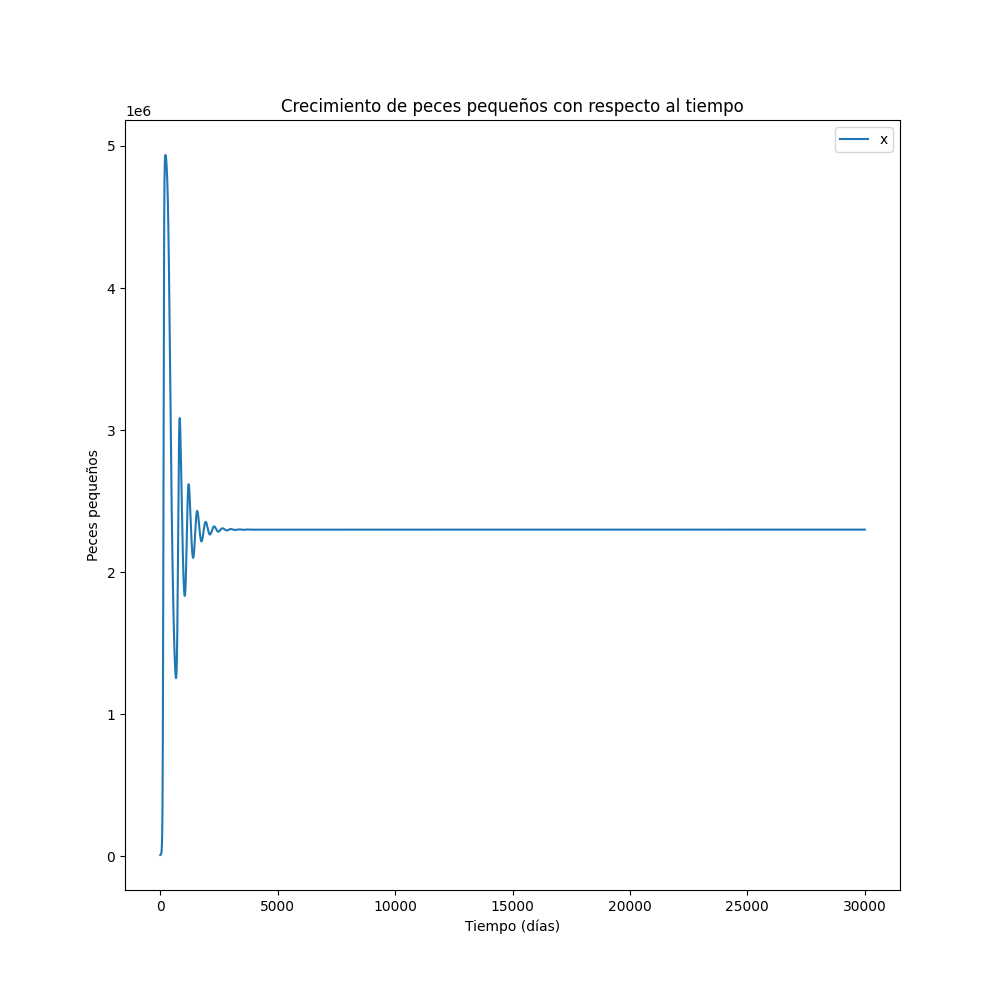
\includegraphics[width=\textwidth, height=\textwidth]{img/Cap-3/apartado-1/peces_pequenos_125.png}
    \caption{Crecimiento de peces pequeños.}
    \label{fig:f1}
  \end{subfigure}
  \hfill
  \begin{subfigure}[b]{0.49\textwidth}
    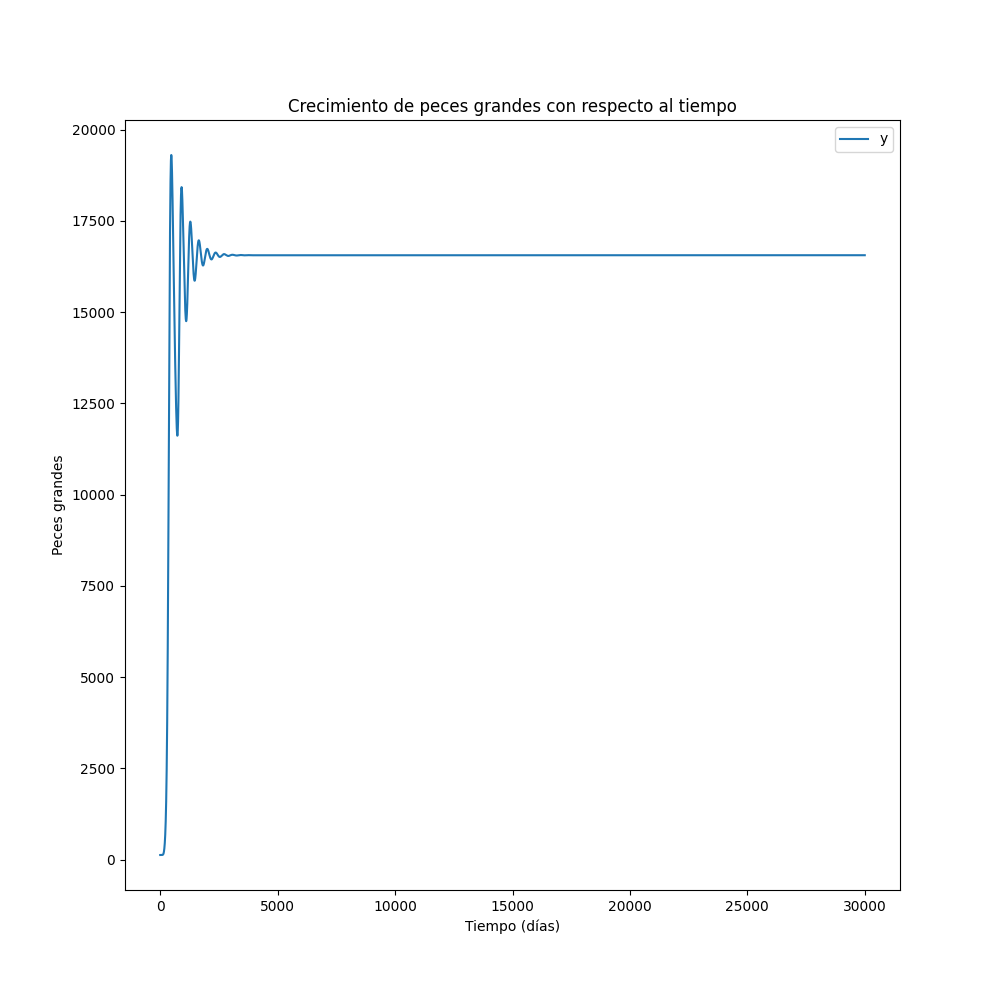
\includegraphics[width=\textwidth, height=\textwidth]{img/Cap-3/apartado-1/peces_grandes_125.png}
    \caption{Crecimiento de peces grandes.}
    \label{fig:f2}
  \end{subfigure}
  \caption{Crecimiento de especies del lago con 10000 peces pequeños y 125 peces grandes}
\end{figure}

\begin{figure}[H]
	\begin{center}
		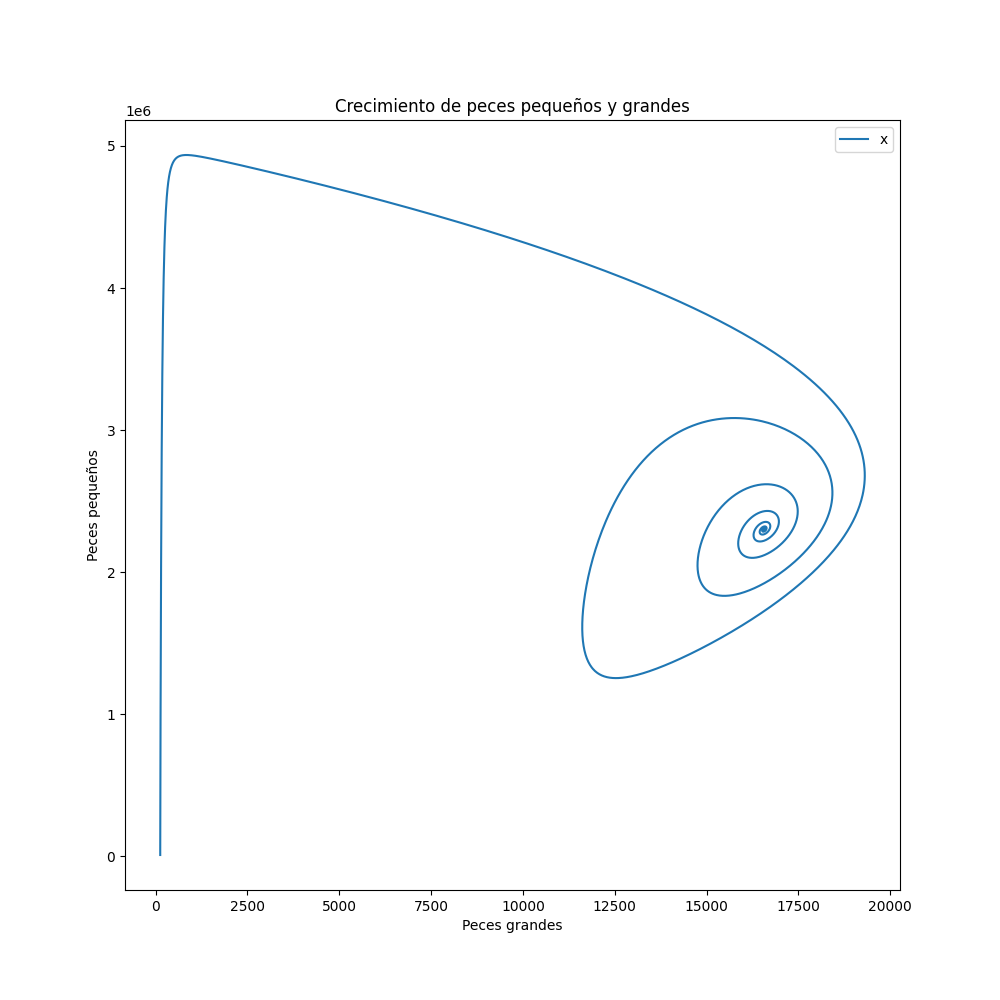
\includegraphics[width=0.49\textwidth]{img/Cap-3/apartado-1/peces_pequenos_grandes_125.png}
		\caption{Comparación entre peces pequeños y grandes al llegar al equilibrio en el lago.}
		\label{fig:f3}
	\end{center}
\end{figure}

En este caso podemos comprobar cómo al principio ambas especies aumentan su tamaño de población de una manera muy rápida y disminuye a los días también pero ambas a la vez, de forma que poco a poco el sistema alcanza un equilibrio donde ambas tienen el mismo valor constantemente debido a que a los peces grandes se comen los peces pequeños al ritmo al que éstos se reproducen.

\section{Campaña de pesca}
Ahora supongamos que planeamos una campaña de pesca para capturar una determinada proporción de peces grandes en la mitad de la simulación. Vamos a comprobar si el sistema se desequilibra al realizar dicha campaña de pesca para tres proporciones distintas: 25\%, 50\% y 75\%.

Empezamos por la pesca del 25\% de los peces grandes:
\begin{figure}[H]
  \begin{subfigure}[b]{0.49\textwidth}
    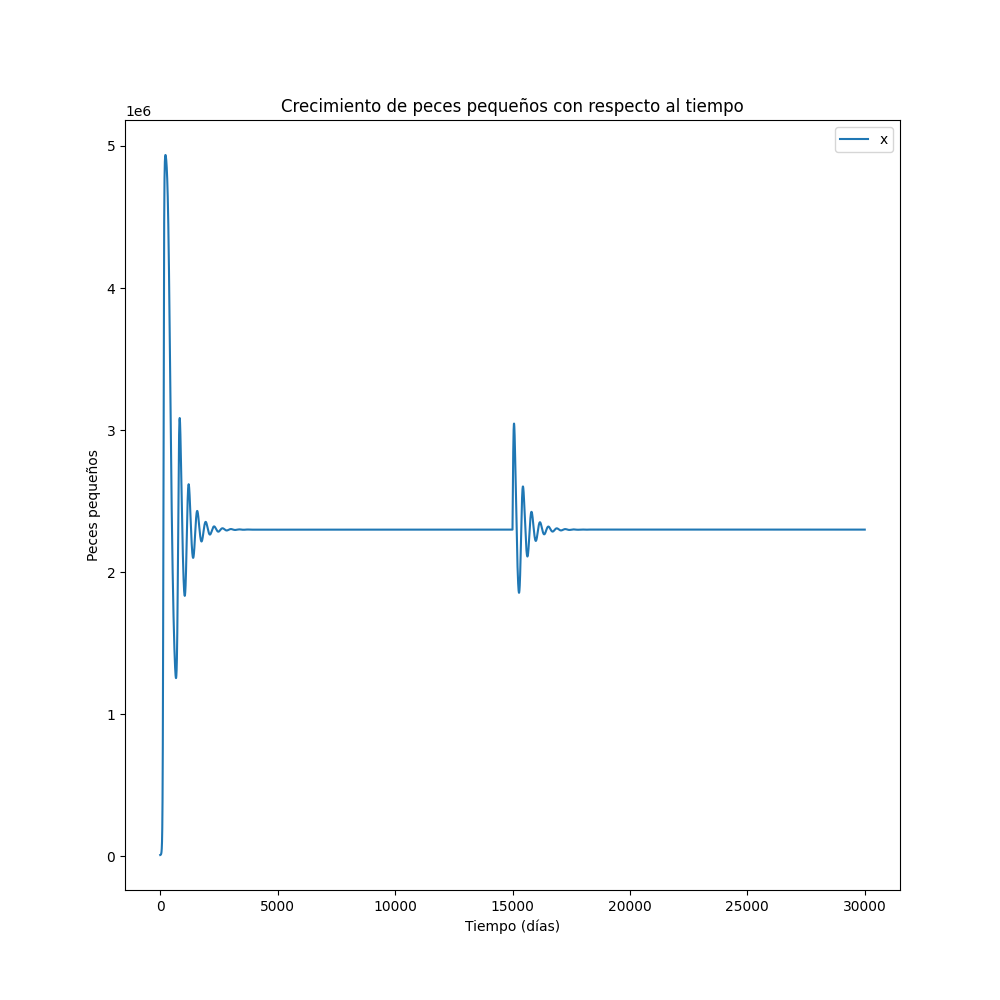
\includegraphics[width=\textwidth, height=\textwidth]{img/Cap-3/apartado-2/pequenyos_pesca_25.png}
    \caption{Crecimiento de peces pequeños.}
    \label{fig:f1}
  \end{subfigure}
  \hfill
  \begin{subfigure}[b]{0.49\textwidth}
    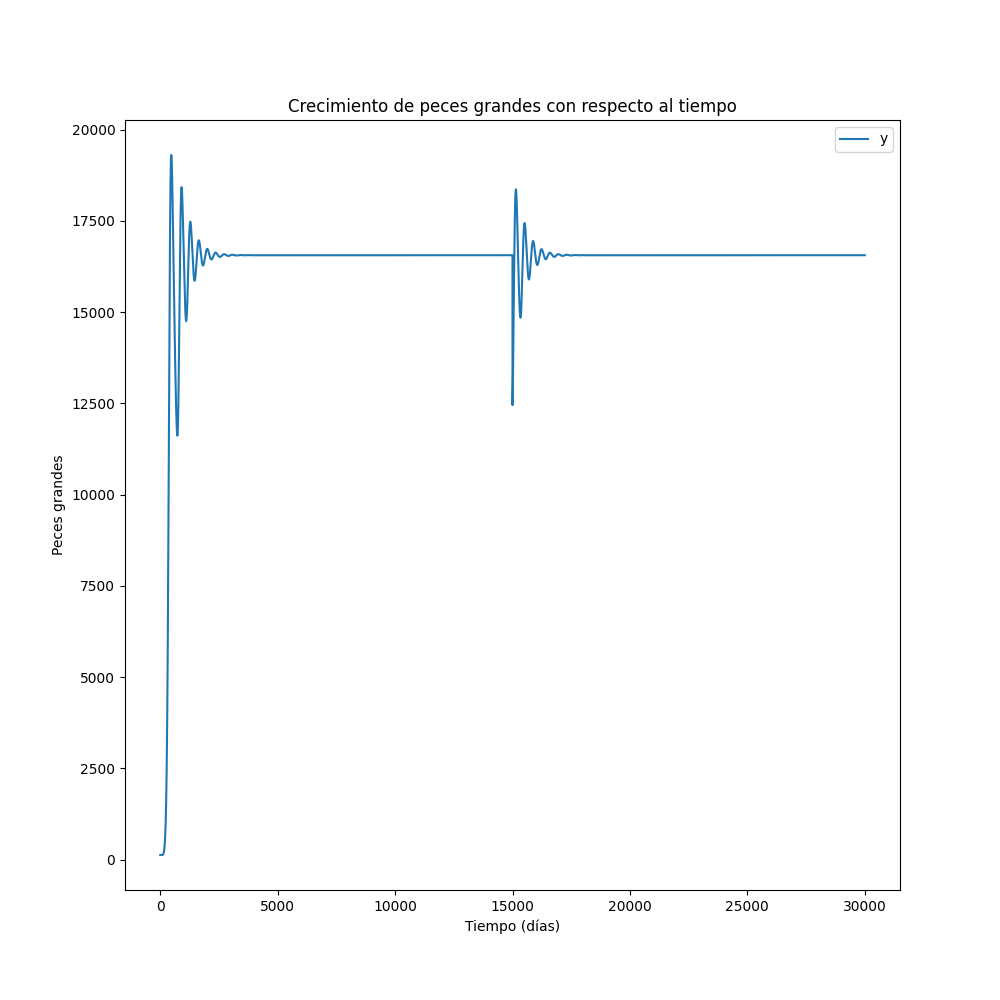
\includegraphics[width=\textwidth, height=\textwidth]{img/Cap-3/apartado-2/grandes_pesca_25.png}
    \caption{Crecimiento de peces grandes.}
    \label{fig:f2}
  \end{subfigure}
  \caption{Campaña de pesca del 25\% de los peces grandes.}
\end{figure}

\begin{figure}[H]
	\begin{center}
		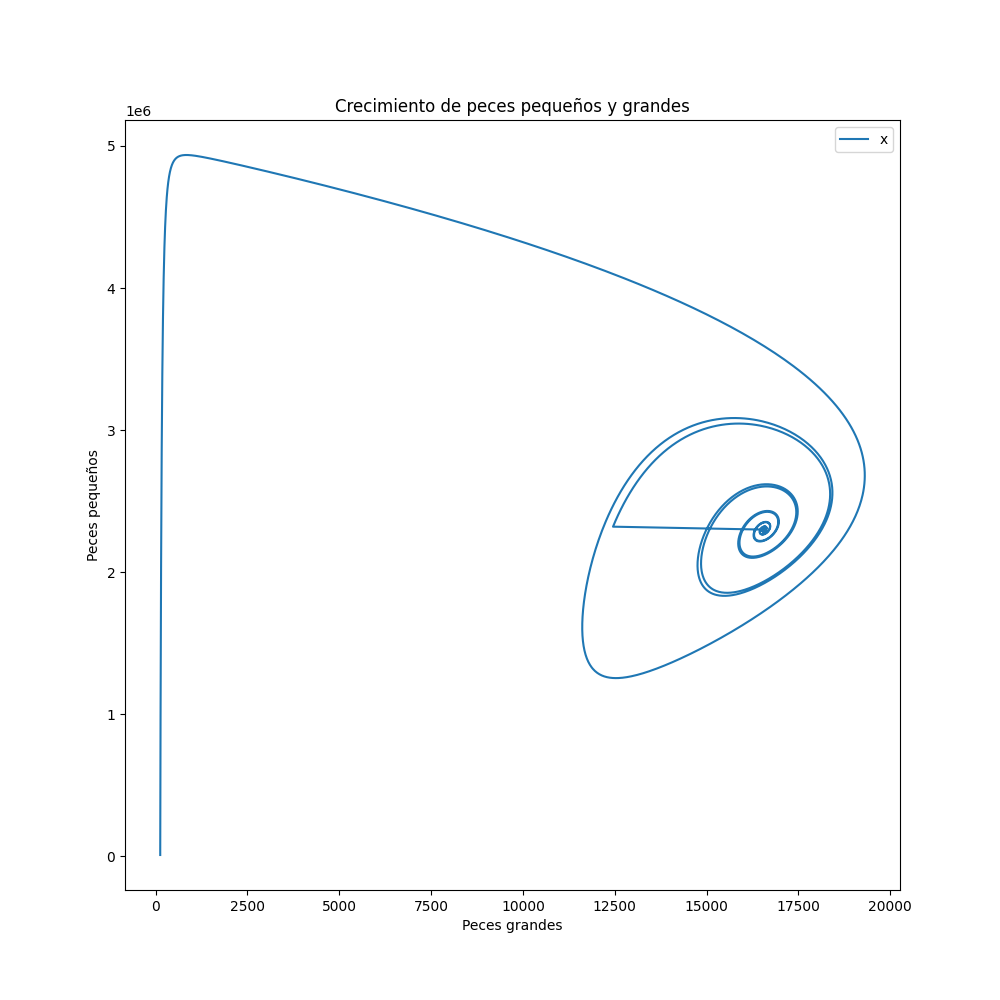
\includegraphics[width=0.49\textwidth]{img/Cap-3/apartado-2/pequenyos_grandes_pesca_25.png}
		\caption{Comparación entre peces pequeños y grandes al llegar al equilibrio en el lago.}
		\label{fig:f3}
	\end{center}
\end{figure}

En este caso vemos cómo al llevar a cabo una pesca de peces grandes, inmediatamente sube la cantidad de peces pequeños en el lago. Pero se puede apreciar cómo la gráfica toma una forma muy similar a la que tenemos en el inicio de la simulación, en la que poco a poco se estabilizan los niveles de ambas especies. Luego el sistema se mantiene en equilibrio.

\newpage
Vamos a probar ahora con el 50\%:
\begin{figure}[H]
  \begin{subfigure}[b]{0.49\textwidth}
    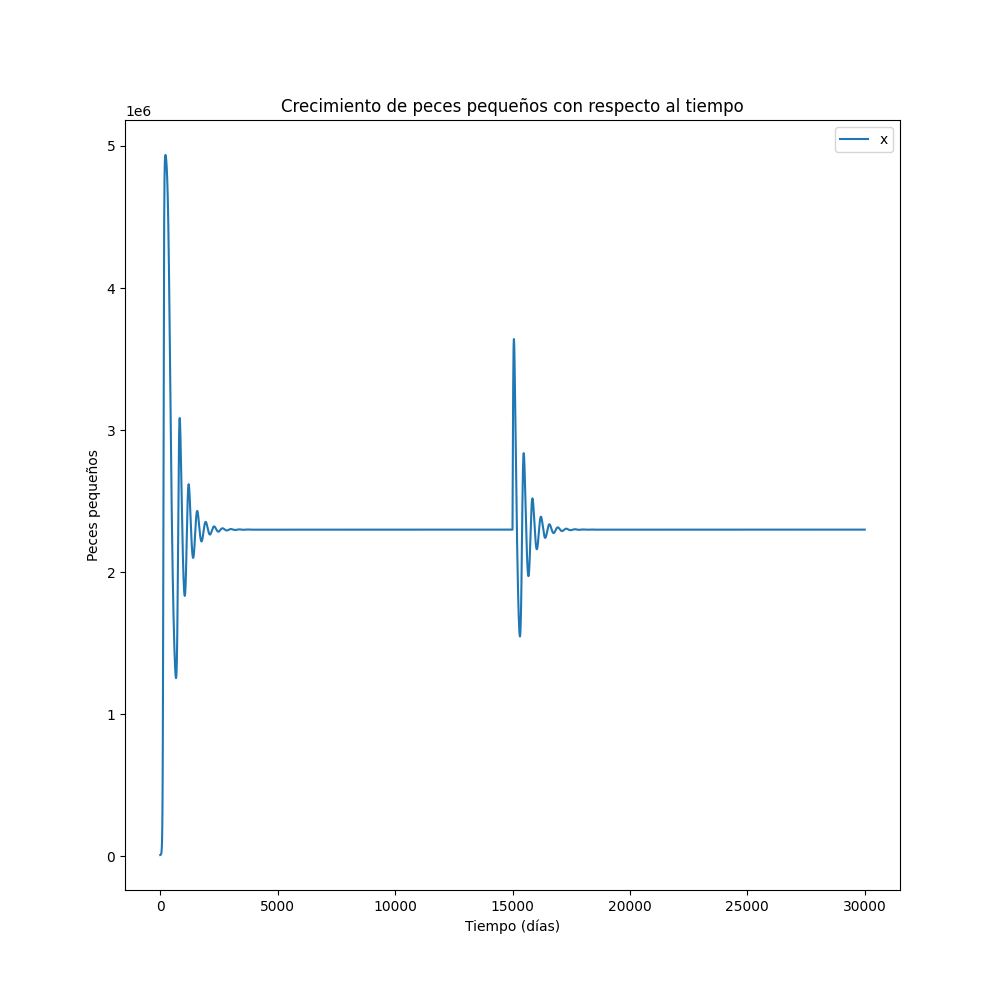
\includegraphics[width=\textwidth, height=\textwidth]{img/Cap-3/apartado-2/pequenyos_pesca_50.png}
    \caption{Crecimiento de peces pequeños.}
    \label{fig:f1}
  \end{subfigure}
  \hfill
  \begin{subfigure}[b]{0.49\textwidth}
    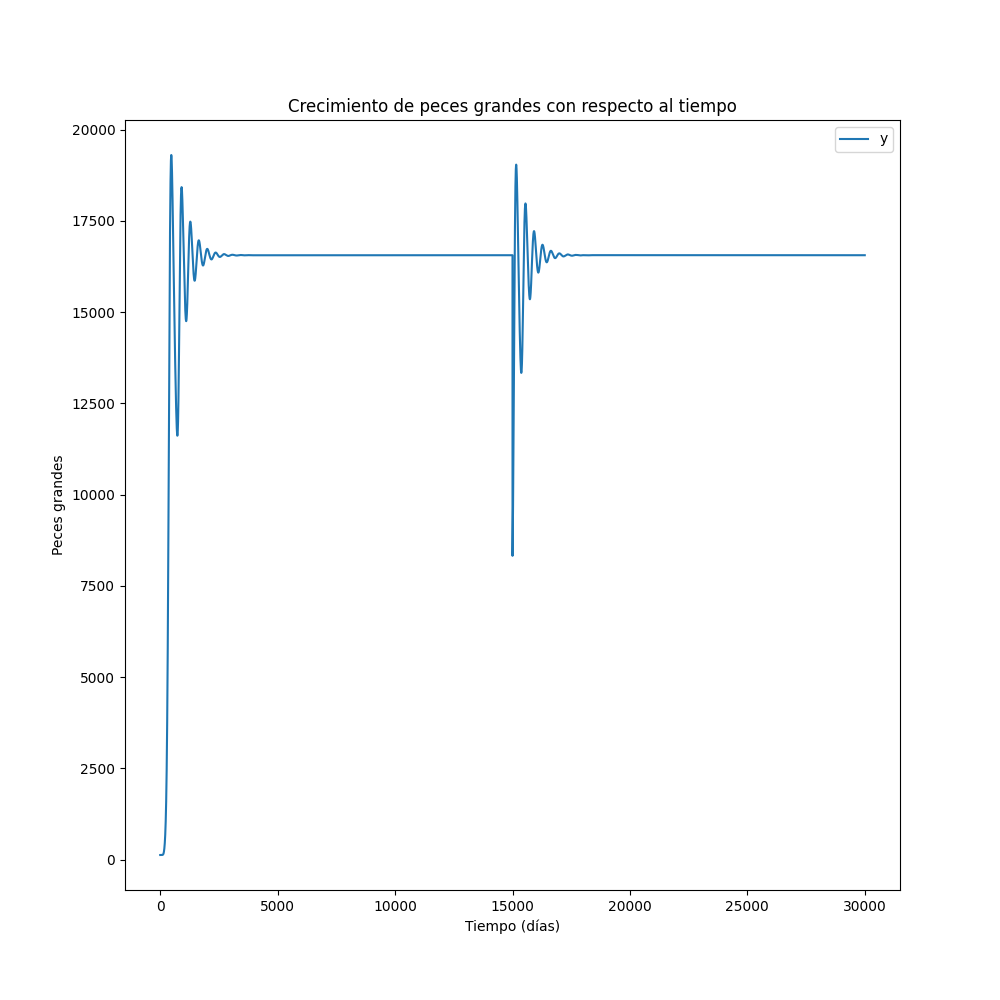
\includegraphics[width=\textwidth, height=\textwidth]{img/Cap-3/apartado-2/grandes_pesca_50.png}
    \caption{Crecimiento de peces grandes.}
    \label{fig:f2}
  \end{subfigure}
  \caption{Campaña de pesca del 50\% de los peces grandes.}
\end{figure}

\begin{figure}[H]
	\begin{center}
		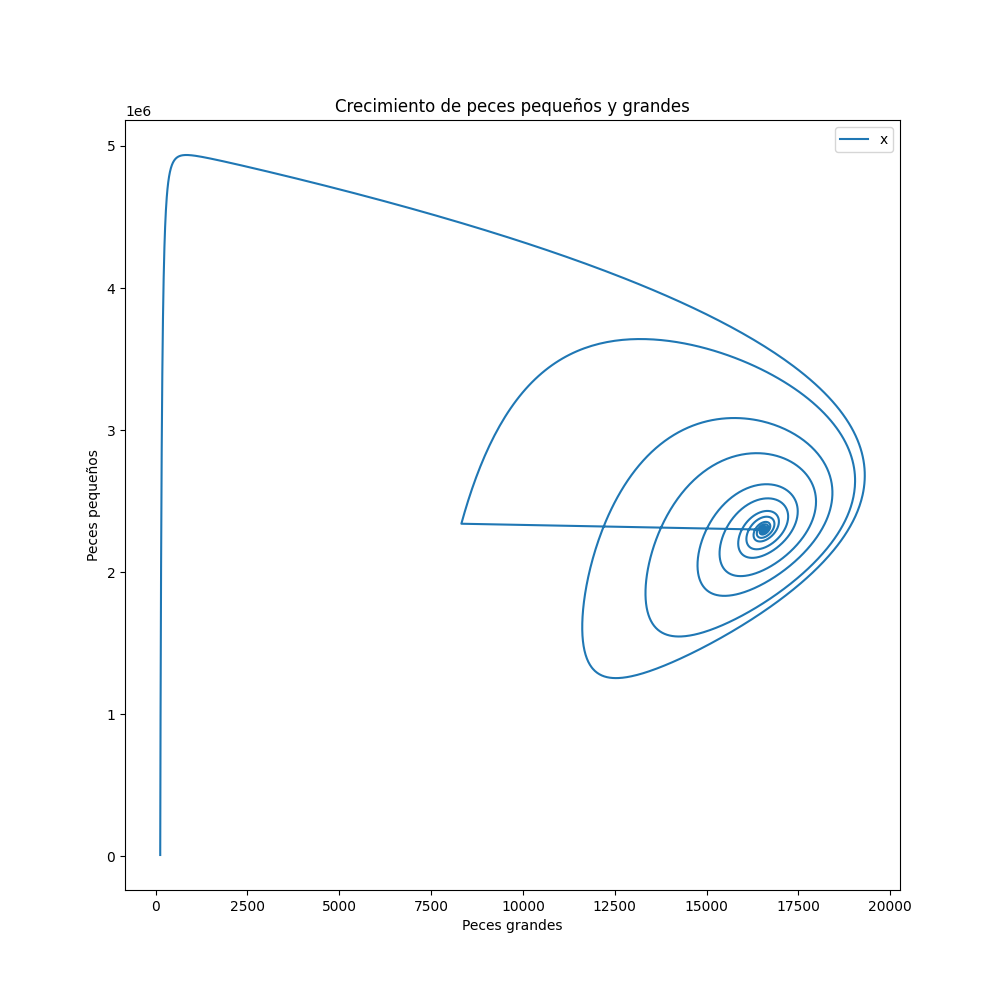
\includegraphics[width=0.49\textwidth]{img/Cap-3/apartado-2/pequenyos_grandes_pesca_50.png}
		\caption{Comparación entre peces pequeños y grandes al llegar al equilibrio en el lago.}
		\label{fig:f3}
	\end{center}
\end{figure}

Podemos ver cómo pasa algo similar al caso anterior. Los peces pequeños esta vez tienen una subida de población más grande al haber pescado más cantidad de peces grandes, pero vuelve a estabilizarse pasados varios años. Luego éste sistema también se mantiene en equilibrio pescando la mitad de la población de peces grandes.

Por último vamos a comprobar qué pasa cuando pescamos el 75\% de los peces grandes:

\begin{figure}[H]
  \begin{subfigure}[b]{0.49\textwidth}
    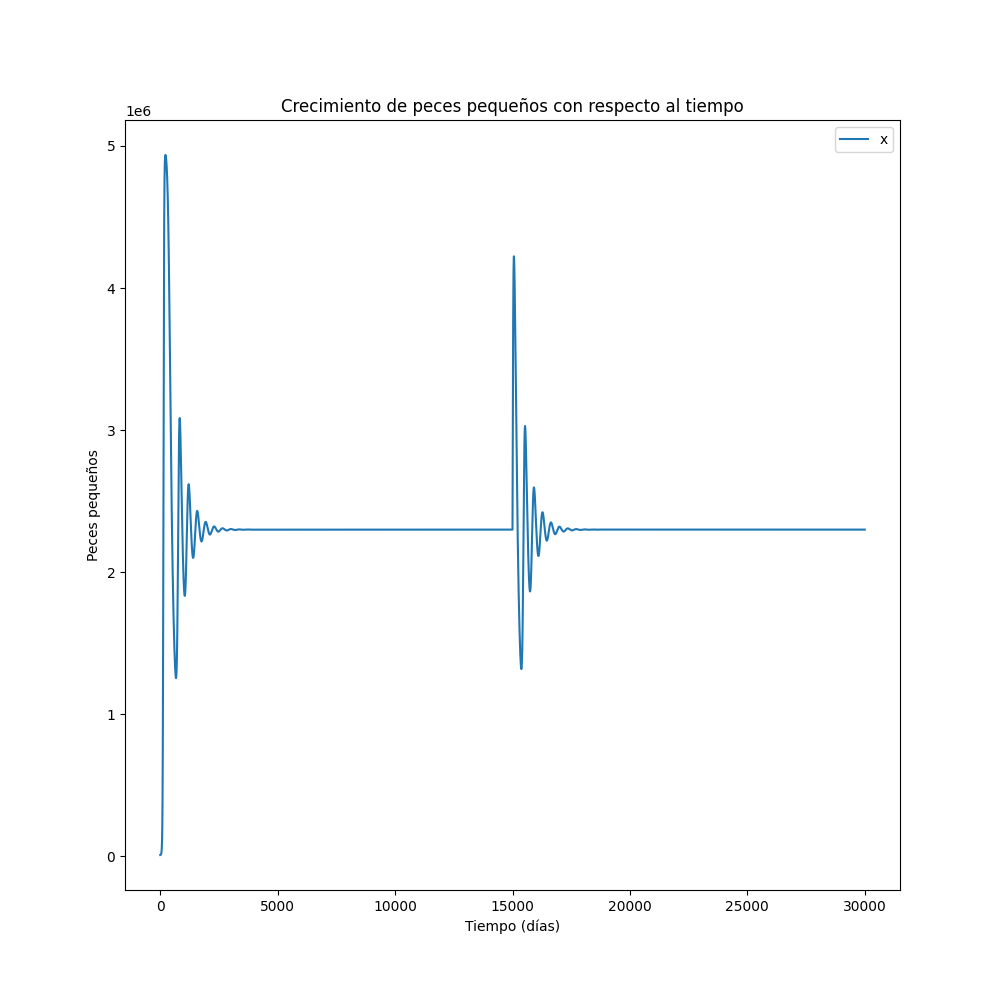
\includegraphics[width=\textwidth, height=\textwidth]{img/Cap-3/apartado-2/pequenyos_pesca_75.png}
    \caption{Crecimiento de peces pequeños.}
    \label{fig:f1}
  \end{subfigure}
  \hfill
  \begin{subfigure}[b]{0.49\textwidth}
    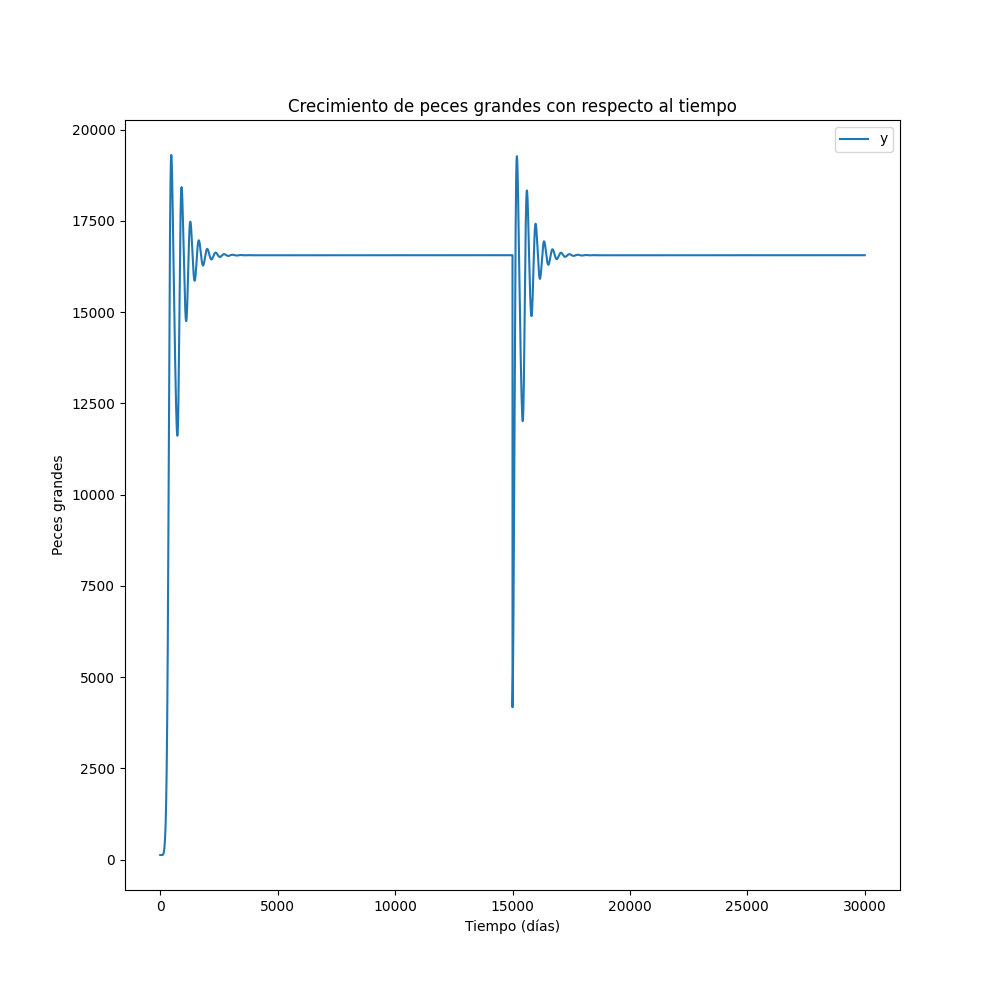
\includegraphics[width=\textwidth, height=\textwidth]{img/Cap-3/apartado-2/grandes_pesca_75.png}
    \caption{Crecimiento de peces grandes.}
    \label{fig:f2}
  \end{subfigure}
  \caption{Campaña de pesca del 75\% de los peces grandes.}
\end{figure}

\begin{figure}[H]
	\begin{center}
		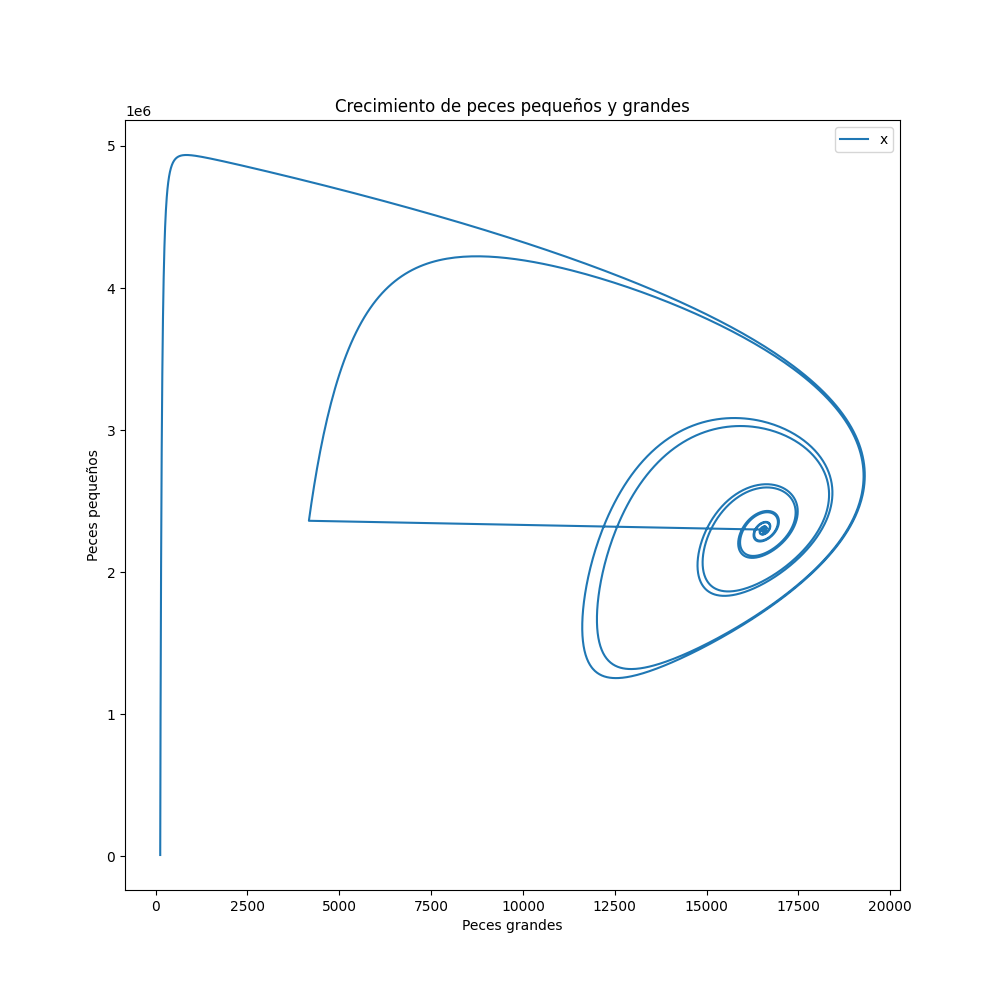
\includegraphics[width=0.49\textwidth]{img/Cap-3/apartado-2/pequenyos_grandes_pesca_75.png}
		\caption{Comparación entre peces pequeños y grandes al llegar al equilibrio en el lago.}
		\label{fig:f3}
	\end{center}
\end{figure}

Podemos comprobar que pasa exactamente lo mismo que para los dos casos anteriores, pero en este caso tendremos un crecimiento más pronunciado de la especie de peces pequeños, y ademas tendrá que pasar más tiempo hasta que el sistema se equilibre de nuevo.

\section{Simulando distintas políticas de pesca}
Por último, vamos a simular qué sucede si planeamos distintas campañas de pesca de peces grandes. Para ello voy a limitar la búsqueda en 5 rangos de periodos que serán: cada 4 meses, cada 6 meses, cada año, cada 2 años y cada 4 años. Vamos a pescar en todos los rangos la misma proporción de peces grandes, que será un 65\% de éstos los que capturaremos (he probado con distintos valores de proporción y he cogido el que mejor resultado me ha dado). Podemos ver las simulaciones en la siguiente gráfica:

\begin{figure}[H]
	\begin{center}
		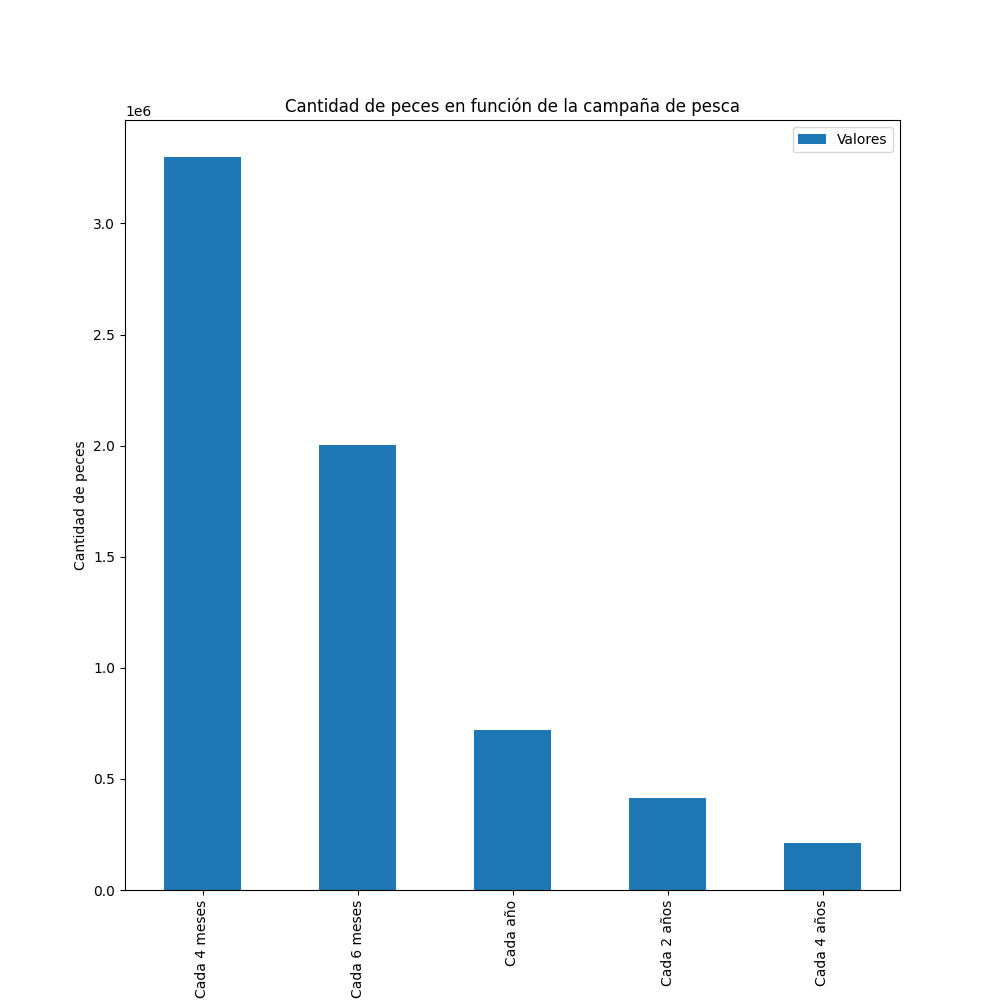
\includegraphics[width=0.8\textwidth]{img/Cap-3/apartado-3/pescados_por_periodo.png}
		\caption{Cantidad de peces pescados al final de la simulación.}
		\label{fig:f3}
	\end{center}
\end{figure}

Podemos ver que a medida que esperamos más tiempo entre pesca y pesca obtenemos menos peces teniendo en cuenta de el sistema no se desequilibra en ninguno de éstos periodos. Como en el tiempo de simulación, la mayor cantidad es la obtenida es la de la campaña cuatrimestral, obteniendo más de 3 millones de peces acumulados. Sabiendo este dato, vamos a profundizar más y vamos a ver las gráficas con respecto del tiempo de qué es lo que pasa con los peces pequeños, grandes y la comparación entre ambos:

\begin{figure}[H]
  \begin{subfigure}[b]{0.49\textwidth}
    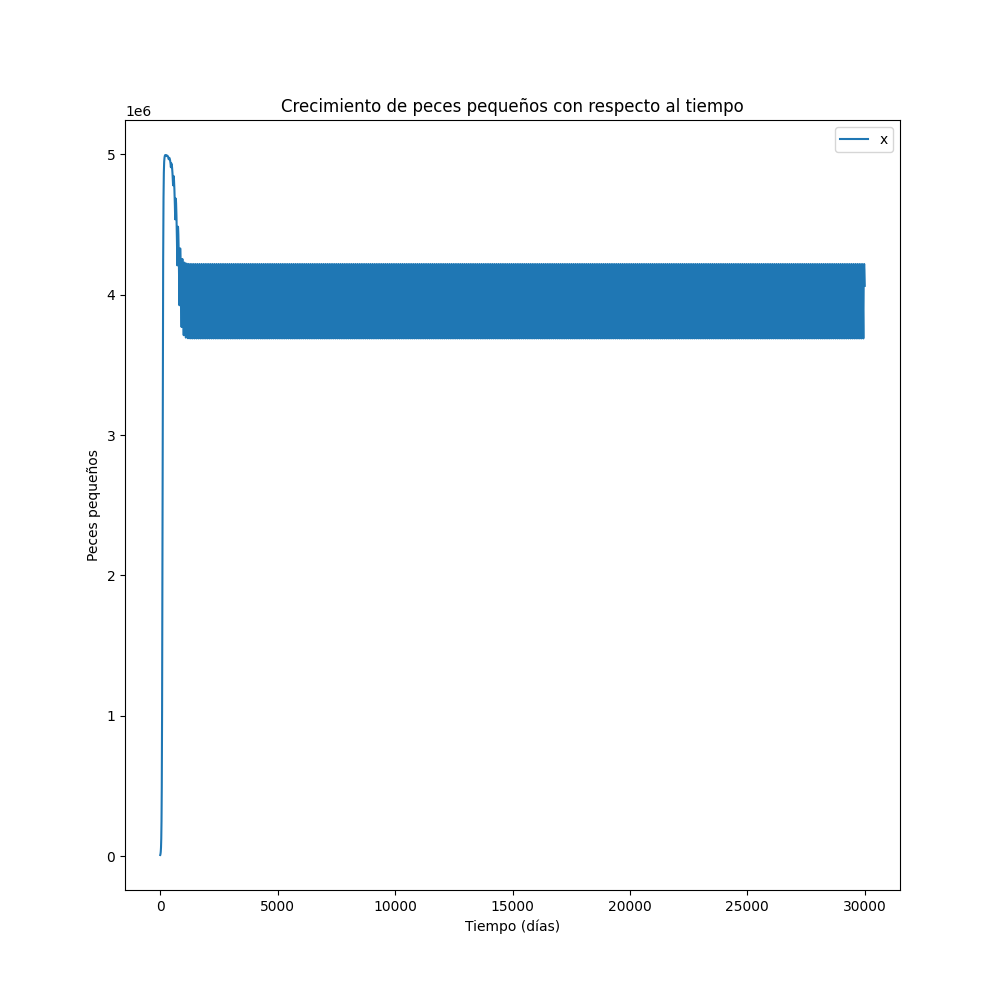
\includegraphics[width=\textwidth, height=\textwidth]{img/Cap-3/apartado-3/pequenyos_periodo_91.png}
    \caption{Crecimiento de peces pequeños.}
    \label{fig:f1}
  \end{subfigure}
  \hfill
  \begin{subfigure}[b]{0.49\textwidth}
    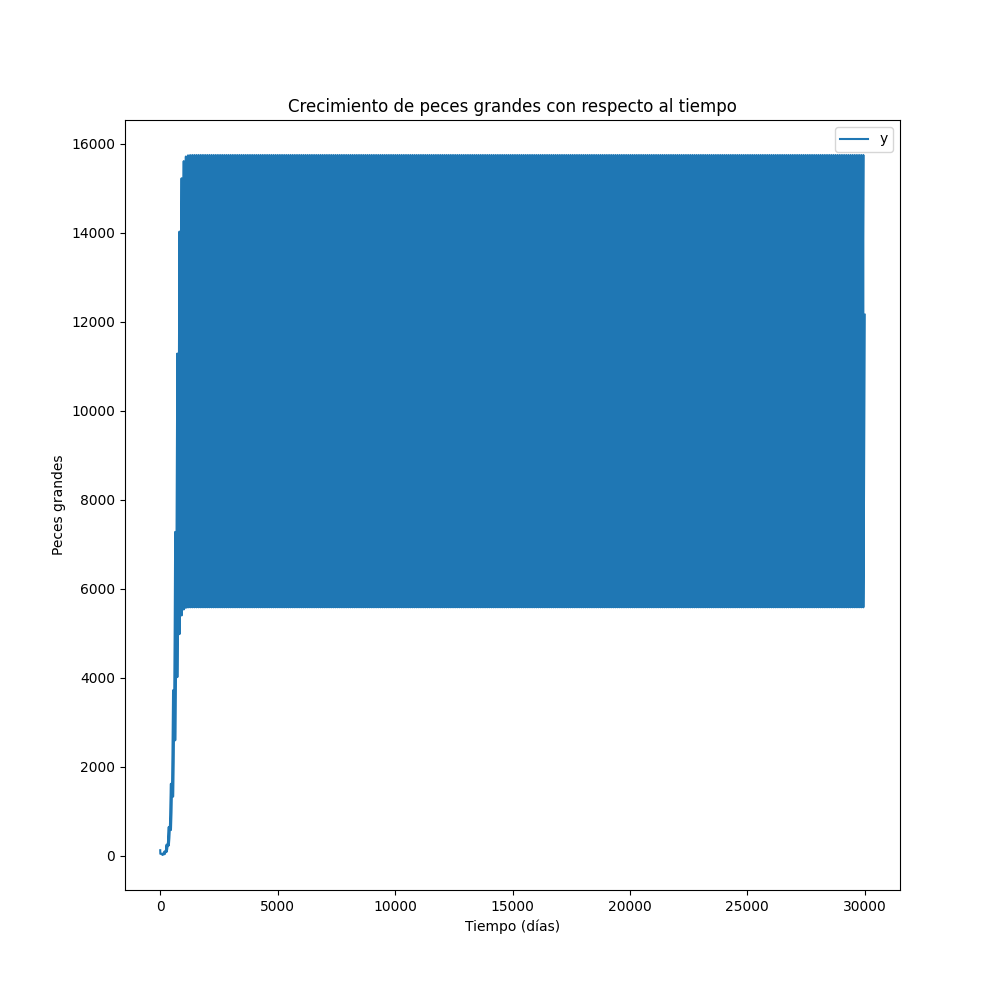
\includegraphics[width=\textwidth, height=\textwidth]{img/Cap-3/apartado-3/grandes_periodo_91.png}
    \caption{Crecimiento de peces grandes.}
    \label{fig:f2}
  \end{subfigure}
  \caption{Crecimiento de especies del lago con pescas del 65\% de peces grandes cuatrimestralmente.}
\end{figure}

En la gráfica del crecimiento de los peces grandes, podemos ver cómo se recuperan rápidamente los peces grandes ante las campañas de pesca, llegando a alcanzar siempre el mismo valor máximo cada cuatrimestre. Por tanto podríamos pescar ésa cantidad de peces grandes sin preocuparnos de que el sistema se desequilibre.

\begin{figure}[H]
	\begin{center}
		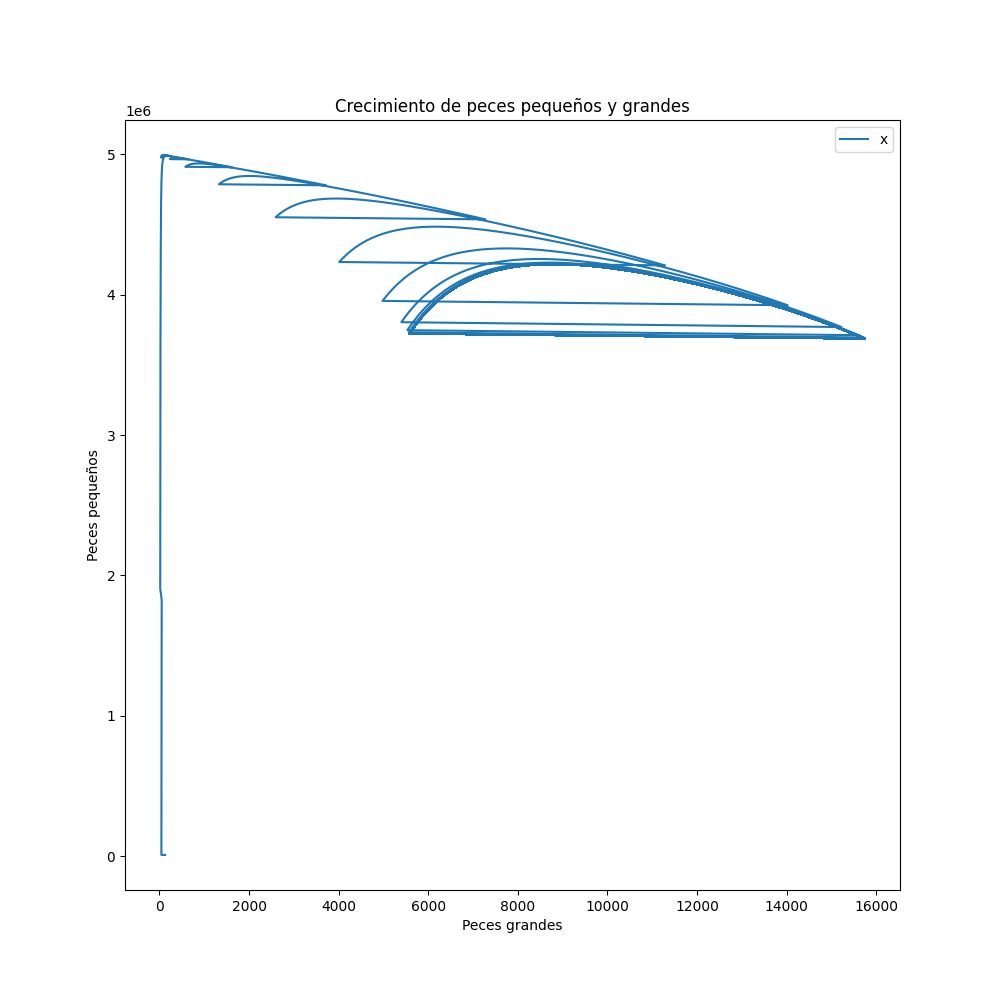
\includegraphics[width=0.49\textwidth]{img/Cap-3/apartado-3/pequenyos_grandes_periodo_91.png}
		\caption{Comparación entre peces pequeños y grandes con pescas del 65\% cada cuatrimestre.}
		\label{fig:f3}
	\end{center}
\end{figure}

En ésta gráfica comparativa entre la cantidad de peces pequeños con respecto de los peces grandes, vemos cómo se hace un dibujo distinto que las anteriores simulaciones. Ésto es porque sigue una forma cíclica en la que tanto los peces grandes y pequeños (cuando se estabilizan los niveles de peces de cada especie en el lago) crecen y decrecen su número en función de las pescas, alcanzando un máximo y un mínimo siempre de forma muy similar al anterior cuatrimestre.

\end{document}

